
\chapter{Radiomics: state-of-the-art}\label{radiomics}

\section{Introduction}\label{introduction}

As explained previously, there are mainly two ways for establishing the diagnosis and the staging of liver cancers: the biopsy and the
diagnostic imaging. The biopsy, as detailed earlier, suffers from a lot of drawbacks. It
remains an invasive procedure, with a high cost in terms of resources,
and does not consider the tumor heterogeneity. The diagnostic imaging on the other hand, is not invasive, provides
information about the tumor shape, the growth over the time, and is less
prone to bias due to tissue heterogeneity.
The biopsy remains the only available ground truth since diagnosis imaging still suffer from the medical expert subjectivity. The biopsy and the medical imaging analysis are currently complementary considering that they provide different information. In our work, we are trying to prove that medical images can be used to improve the visual inspection of the medical expert and at long-term replace invasive procedure such as the biopsy.\\
The improvements in the medical imaging field allow acquisition
of data enabling a better characterization of the patients phenotype. In the case of brain imaging, the augmentation of contrast, on MR
images, thanks to the injection of contrast agents such as
gadolinium-based agents (method mentioned before) is an important
technique for the evaluation of brain and liver tumors \cite{Drevelegas2011,Zhou2014,Thian2013}. This tool allows a delineation of large tumors and an
early detection of small metastatic lesions. The different MRI sequences
(e.g. the T1 weighted sequences) also allow an internal separation of
the tissue within the same tumor (active vs necrotic part of the tumor)
\cite{Drevelegas2011}. \\
Support brought by the innovations in the medical imaging field have
been demonstrated on other organs such as the liver \cite{Davnall2012}, the breast \cite{Koolen2012} or the colon
\cite{Sahani2014} with a consequent benefit in terms of
diagnosis. However, even though the advancements in the medical imaging fields have
allowed these performances, the interpretation of the medical images
remains subjective and not quantitative. In order to improve the quality of the diagnostic, it is important to decode the information present in the image, often difficult or impossible to assess with the naked eye (such as textural-based information).

Introduced in the 80s, CAD (\emph{Computer Assisted Diagnosis}) tools
were the first to establish a link between the
imaging features and the biological characteristics of the patients
\cite{Doi2007}. In order to go along with those new systems, standards were introduced
such as the one created by the WHO (\emph{World Health Organization}) 
or the RECIST (\emph{Response Evaluation Criteria in Solid Tumors})
\cite{Jaffe2006}, where the objective was to assess the
evolution of the disease following the progression of the tumor size,
but here again, those criteria suffer from a too high dependence with
the observers.\\
The term \emph{radiomics} was introduced in the early 2010s, allowing
the computation of more features than the traditional CADs (more
than a thousand vs only a dozen previously) and bringing a more complete
diagnosis, since CADs were often limited to distinguish benign vs
malignant lesions \cite{Afshar2018}.
This new technique allows some breakthroughs in various applications
such as the cancer diagnosis, the detection of the tumors (with the
identification of malignant lesions), their classification, the
estimation of the patient survival, the prediction of the aggressivity
of the tumors, their recurrence, or the advancement of the disease.
In the clinical practice, this new method also allows an improvement in
the way biopsies are performed, with the identification of the areas
where the extraction should be performed \cite{Gillies2016}
or even by predicting when a biopsy is helpful or not \cite{Liu2016}.\\
Compared to the above-mentioned criteria based on a naked-eye examination,
we are now able to rely on a computer to analyse the gray-levels at a
finer scale. Therefore, two approaches exist, the \ac{hcr} (\emph{Hand-Crafted
Radiomics}) based on mathematical engineered features, relying on the
textural, intensity and shape based properties of the volume of interest, and
the \ac{dlr} (\emph{Deep-Learning radiomics}), where the extracted features
are estimated from the input data without any prior
knowledge.

\section{Handcrafted Radiomics }\label{handcrafted-radiomics}

In this section we will describe the \ac{hcr} pipeline, by first
exposing the different steps of the classical workflow, before analyzing
the different studies that used \ac{hcr} on patients suffering from
HCCs. We will conclude with the different improvements that
should be brought to enhance the predictive value of radiomics.

A conventional radiomics workflow (based on \ac{hcr} features) starts
with the acquisition and the reconstruction of medical images, followed
by the segmentation of those images, which is a critical step since
\ac{hcr} features are extracted from organs or lesions having indistinct borders \cite{Gillies2016}. 
Once the different areas were segmented, the features are
extracted and quantified, and a statistical analysis is performed to
select only the most relevant one. The final step consists in building a
model that use the selected features to perform the wanted task,
which is often either the tumor characterization or its prognosis. The
pipeline is illustrated in the figure below \ref{Scrivener2016_Fig1}.


\begin{figure}[th!]
\centering
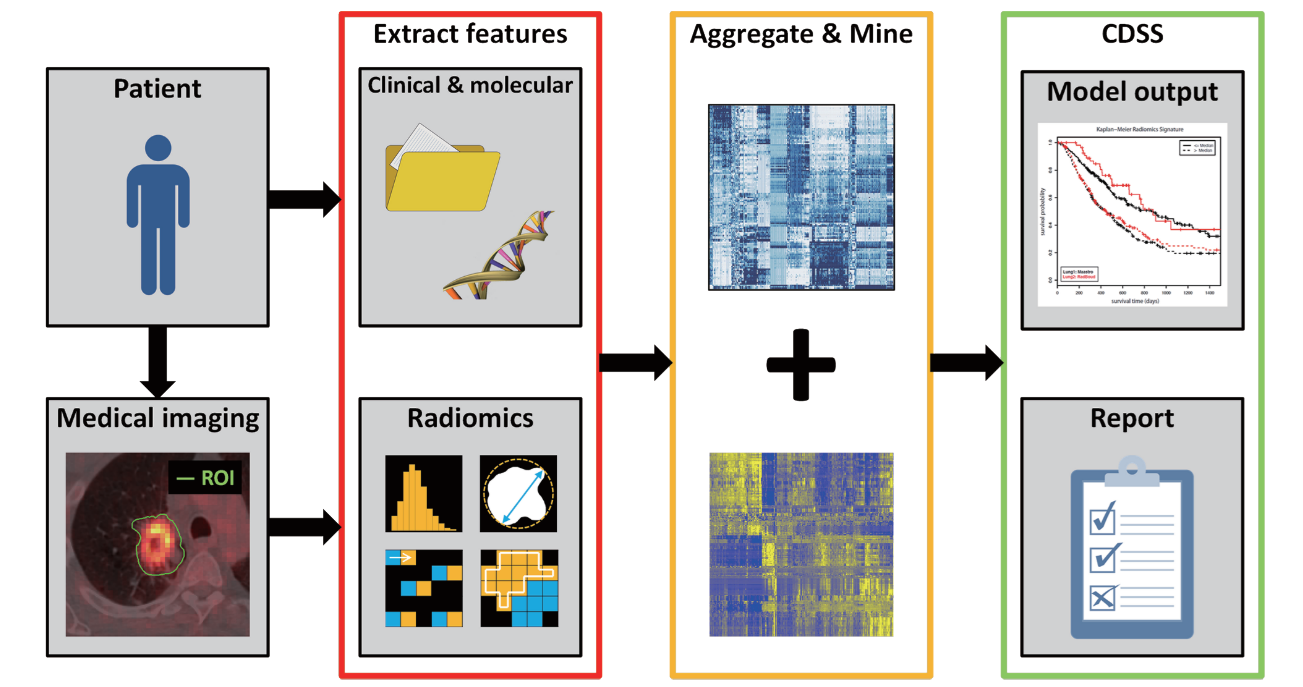
\includegraphics[width=0.7\linewidth]{images/image4_crop}
\caption{Conventional radiomics workflow as depicted by \textbf{©Scrivener et al.} \cite{Scrivener2016}}
\label{Scrivener2016_Fig1}
\end{figure}


We will now describe these different steps, before analyzing recent
state-of-the-art \ac{hcr} studies, before establishing a list of
measures needed to be taken in order to improve the quality and the
reproducibility of future radiomics works.

\subsection{HCR workflow}\label{hcr-workflow}

\subsubsection{Image acquisition and reconstruction}\label{image-acquisition-and-reconstruction}

As explained previously (see chapter \ref{liverCancer}), ultrasonography (US) is the recommended
modality as primary imaging test for surveillance. If the surveillance
is positive, CT or MR examinations are performed for the diagnosis and
the staging of the disease. For the reasons exposed previously, namely
the availability, and its robustness when compared to MRI, we will focus
on \ac{hcr} studies based on CT imaging data.\\
Without entering into the details of how a CT scan works, we can assume
that performances of the CT imaging depend mainly on some settings such
as the slice thickness, the capability for projecting the density
variations into image intensities and the reconstruction algorithm which
aims at converting tomographic measurements into cross-sectional images.
It has been demonstrated that radiomics features can differ between
different scanners with the same settings \cite{Berenguer2018}. 
It is also common to differentiate CT images into two
categories, the screening where low dose images are used and the
diagnosis with higher quality of contrast obtained with 
higher doses \cite{Thawani2018}. The investigated studies aim for the diagnosis of the disease, therefore higher doses were used during the imaging acquisition.\\
Images are typically combined with other clinical sources when computing
the radiomics features. Among them, gene expressions, clinical data such
as the age, the gender or the past medical history, blood biomarkers or
other prognostic markers such as the tumor size, the stage or the
recurrence are the main non-imaging sources of data that are used in the
radiomics workflow. However, they can be difficult to acquire, normalize
and integrate in a radiomics pipeline, therefore, features are most
commonly extracted from images only.

\subsubsection{Segmentation}\label{segmentation}

Historically, the segmentation was performed manually, hence, prone
to the inter- and intra-observer variability, as depicted below in the figure \ref{Bakr_Fig2}.
%\begin{figure}[th!]
%	\centering
%	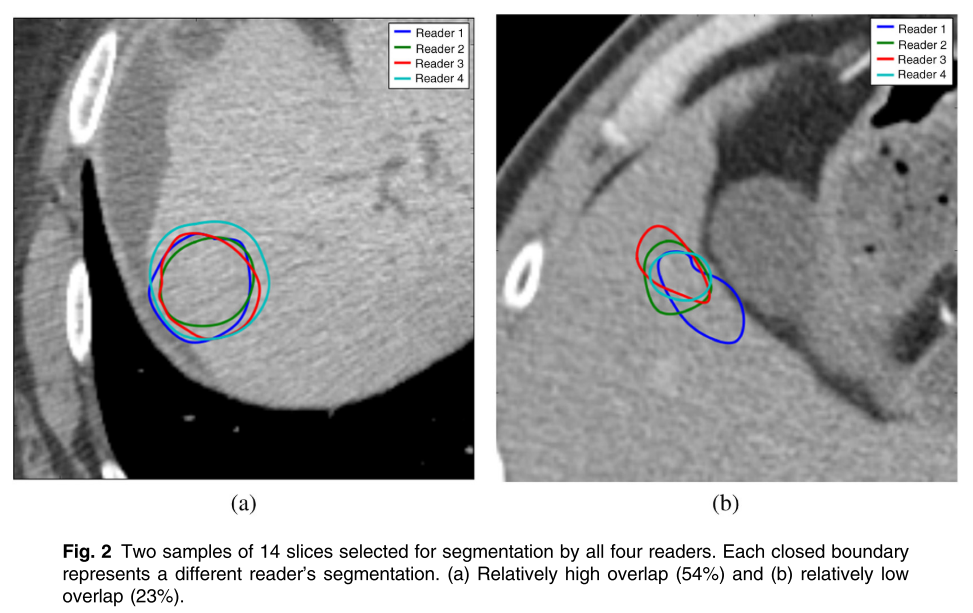
\includegraphics[width=0.7\linewidth]{images/image11}
%	\caption{Inter-observer variability in the tumor segmentation, as reported by \textbf{© Echegaray et al.} \cite{Echegaray2015}}
%	\label{Echegaray_Fig2}
%\end{figure}

\begin{figure}[th!]
	\centering
	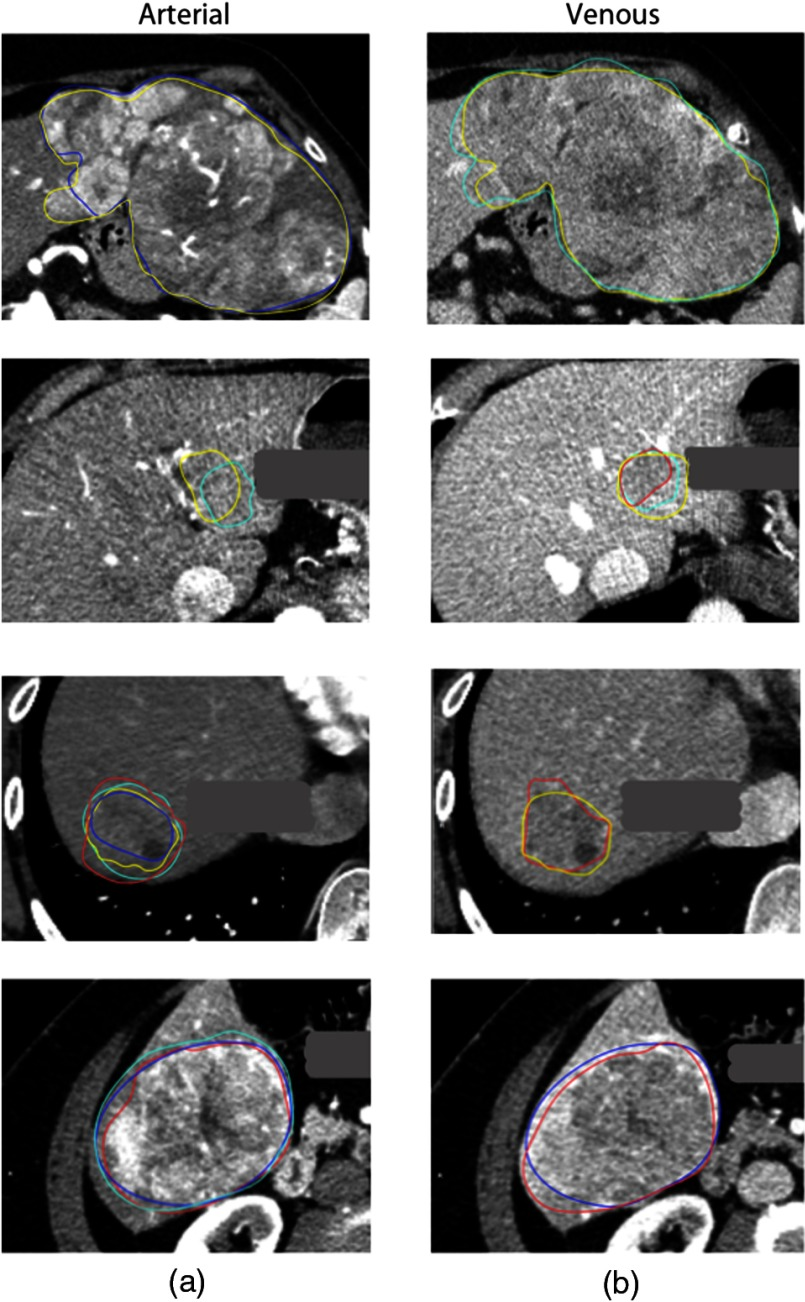
\includegraphics[width=0.7\linewidth]{images/image14}
	\caption{Inter-observer variability between 4 different observers on multiphasic images ((a) corresponding to arterial phase images and (b) to portal venous phase images), with a dice similarity coefficient from 0.19 to 0.93, \textbf{©Bakr et al.} \cite{Bakr2017}}
	\label{Bakr_Fig2}
\end{figure}


To reduce this bias, automatic segmentation techniques were
developed. These techniques based on the intensity of the pixels suffer from the
fact that the intensity of the pixels, in the case of abdominal organs,
is often close from one organ to another. On the other hand, models
based on statistical representations often require the computation of an energy
function, that can involve a large number of parameters, thus being
difficult to compute and optimize (more details concerning the liver semantic 
segmentation techniques are given in the chapter \ref{SegSemantic}).\\

\subsubsection{Features}\label{features}

Once the volume of interest is delineated, different features can be
extracted. On one hand, features can be chosen a priori for their
ability to translate the physiological behavior expected by the
experts. For example, studies performed on the lungs showed a
correlation between the textural homogeneity and the survival of the
patients \cite{Ganeshan2012,Balagurunathan2014}, or the grade
\cite{Al-Kadi2008}. This knowledge can also be used in the case of
brain tumors to assess the response to a treatment, by observing for
example the vascular or cellular density \cite{Cao2006,Zhou2014}. 
However, a prior knowledge is not always available for the wanted
task, therefore, the alternative is to extract a huge quantity of
features and to determine the most relevant one by using for example
some machine learning algorithms.\\
Features can be regrouped into different categories depending on their
statistical order (first, second or higher order). For the features
belonging to the first statistical order, the intensities of the volume of interest are 
summarized by an histogram, and different values are computed such as
the uniformity or the entropy. Even though these features are often
sensitive to the acquisition settings and by the way the histogram is computed, they already permitted the prediction of
the malignancy of breast lesions \cite{Parekh2016}.\\
Second order statistical features are meant to extract the textural
properties of the volume, by considering the neighboring relationship
between pixels. This will play an important role especially for the
characterization of the heterogeneity of the tissues. This relation is
captured by several descriptive matrices (\ac{glcm}, GLRLM,
\ldots{}) \cite{Parekh2016}.\\
Shape features are often extracted directly from the \ac{voi} in order to
analyze its geometrical properties (such as the overall volume occupied
by the tumor, its sphericity, its roughness or its fractal dimension).
Those features also permitted the prediction of the response to
treatment in previous studies \cite{Thawani2018}.\\
Finally, higher order features allow the extraction of imaging features
in various frequency domains (the Wavelet features are the most commonly
used higher order features \cite{Thawani2018}).

\subsubsection{Features Selection}\label{features-selection}

As listed here, a large quantity of features can be extracted and they
tend sometimes to be highly correlated. The important number of extracted features can often cause
overfitting during the creation of a predictive model. A features reduction
phase is often required, either in a
supervised manner (features are selected for their discriminant power in
regards with the wanted task) or in non-supervised manner (the main
objective is to suppress the redundant features without considering the
different labels) \cite{Parekh2016}.\\
Among the supervised methods, one can distinguish the univariate ones,
where the features are tested one by one depending on their contribution
to the final decision (Wilcoxon or Fisher test), from the multivariate
where the features are regrouped into subsets before being tested
against the output class (such as the Wrapper or the Embedded methods).\\
Unsupervised methods (such as the \ac{pca}: \emph{principal component
analysis}) do not consider the label of the data and try 
to reduce the dimensionality of the features space, however the new principal component are difficult to interpret.\\
Once the number of features is reduced, the next step is to construct a
predictive model, by using either clustering methods (patients are
regrouped based on a metric depending on the retained features, but their label can not be inferred from the clustering) or
classification ones (where models such as RF: \emph{random forests} or
\ac{svm}: \emph{support vector machines} are trained from the selected
features in order to predict the wanted clinical criteria). Concerning
the prediction of the survival, it is common to implement slightly
different models such as the \emph{Kaplan-Meier} or the \emph{Cox
Proportional Hazard} \cite{Oikonomou2018}.

In the radiomics studies, one of the main goals is the stability of the
features against the preprocessing steps described above. In order to
reach this objective, it is possible for the patients to undergo the
medical imaging examinations several times (\emph{test-retest}), and the
segmentations can be performed by several experts or even by the same
expert several times \cite{Griethuysen2017}.

In summary, when dealing with classical radiomics pipelines, reaching
the best results will often depend on the best combinations between the
extraction of the features, the technique used to reduce the number of
features and the method implemented to create the model.
Every modification on the cited steps can have a huge impact on the
predictable performances of the created model.

In the next section, we will analyze the different \ac{hcr} studies
performed on patients suffering from HCC and who underwent CT
examination. We will first describe the different choices made in each
step of the classical pipeline, before presenting ways to improve the
quality of future \ac{hcr} work.

\subsection{\ac{hcr} applied to the HCC}\label{hcr-applied-to-the-liver}

In order to analyze the different methods implemented in the \ac{hcr}
field, we reviewed 15 studies performed on patients suffering from HCC and who
underwent CT scan examination. Initially, 23 primary liver
cancer-related studies have been scanned in our review \cite{Wakabayashi2019}, 
we then selected the 15 HCC-related ones.\\
We will first describe the different targets of the studies and the
details of the cohorts through the number of patients and the clinical
criteria that preceded their selection.
We then compare the different imaging acquisition protocols, and
the way the regions/volumes of interest are delineated. Finally, we will
analyze the different features that appeared to be relevant in the
studies, before proposing some tracks to improve the reproducibility and
the performances of future radiomics work.\\
Details concerning the experimental settings of the studies, the
endpoints and the different retained features can be found 
in the table \ref{tab:HCR_studies_details}.

\renewcommand{\arraystretch}{1}
\newgeometry{vmargin={15mm}, hmargin={10mm,10mm}}
\begin{landscape}
   % set the margins 
\small

\begin{longtable}{p{2cm}|p{1.5cm}p{1cm}p{2cm}p{2cm}p{2cm}p{2cm}p{2cm}p{2cm}p{1.5cm}p{2cm}p{1cm}}
\textbf{Author} &\parbox{2cm}{\textbf{Modality \\ \& slice \\thickness}} &\parbox{2cm}{\textbf{Mean \\tumor\\ size}} &\textbf{Treatment} &\textbf{\#Patients + Inclusion Criteria} &\textbf{Segmentation} &\textbf{\#Computed features} &\textbf{Retained features} &\textbf{Retained features category} &\textbf{Study endpoints} &\textbf{Results} &\textbf{\% RQS (points)} \\ \hline \endfirsthead
Cozzi et al. \cite{Cozzi2017} &NECT 3 mm &- &Radiotherapy (volumetric modulated arc therapy) &138 Patients with BCLC stages from A to C, Child-Pugh stages A-B &Segmentation done using the CTV (clinical target volumes) which is manually contoured (whole tumor analysis) &35 extracted features * 6 geometry and histogram based features * 6 GLCM * 2 NGLDM * 11 GLRLM * 10 GLZLM &Compacity (shape-based feature) , Energy (histo-based) and GLNU &Quantitative &OS \& local control of the tumor after radiation treatment &* AUC of the model is 0.80 * Survival could be predicted using a radiomics signature made by a single shape-based feature. &14 (5) \\ 
Zhou et al. \cite{Zhou2017a} &Contrast CT (30 and 60s) 1.25 mm &- &Hepatectomy &215 Patients who underwent partial hepatectomy &Largest cross-sectional area of the tumor, manual delineation - exclusion of necrosis 2 experts &300 features * Mean, SD, Kurtosis, Skewness * Percent Mean and SD * 5 features from 4 GLM &Radscore uses histogram features (skewness, energy, means...) &Quantitative &Recurrence &* Radiomics signature using first-order statistical features combined with clinical factors was a good predictor of early recurrence after surgery &25 (9) \\
Akai et al. \cite{Akai2018} &Contrast CT (27-28, 40 and 90 s) 5 mm &3.7 cm (2.4 - 7.0 cm) &Hepatectomy &127 patients &Manually setting the region of interest to include the tumor within the slice at its max diameter. Single radiologist &96 features (mean, sd, positive calue pixels, entropy, kurtosis, skewness) &Entropy and histogram-based features (skewness and kurtosis) &Quantitative &OS and DFS &First-order statistical features were sufficient to predict postoperative survival &25 (9) \\
Chen et al.  23 &Contrast CT (25 and 70s) 1.25 mm &- &Hepatectomy &61 patients with only one lesion and prospective survival above 3 months &ROI was delineated around the tumor outline at the longest dimension (2 experts) &84 features * 12 Gabor * 9 Wavelet * 7 GLCM &* Textural features * Gabor and Wavelet as key features &Quantitative &OS and DFS &Tumor prognosis could be predicted using Gabor and Wavelet responses &17 (6) \\
Li et al.  24 &Contrast CT (70s) 1.25 mm &8.0 cm (5.1 - 18.7 cm) &Hepatectomy or TACE &130 patients 86 treated by LR and 22 by TACE &A user-defined irregular ROI was drawn manually around the largest-cross sectional tumor outline by each expert 2 radiologists &27 features (Wavelet) &2 Wavelet features correlated with survival &Quantitative &OS and Treatment sensitivity &Wavelet features were correlated with post operative survival suggesting a suitable treatment choice &19 (7) \\
Raman et al.  26 &Contrast CT (25s) 3 mm &* Adenoma 7 $ \pm $ 3cm * FNH 6 $ \pm $ 3 cm * HCC 8 $ \pm $ 3cm &- &80 patients 17 FNH 19 Adenomas 25 HCCs 19 normal livers &ROIs were selected from multiple axial slices (from 5 to 10 slices) 2 observers &32 features (mean, SD, entropy, skewness, kurtosis) & SD and Mean of histogram &Quantitative &Diagnosis &A model created using exclusively first-order statistical features was able to differenciate 3 types of hypervascular lesions. (They reached 15\% of error rate) &3 (1) \\
Kuo et al.  29 &Contrast CT (30-35 and 60-70s) 2.5 mm &- &- &30 Patients * no patients included received chemo before resection &No segmentation, Images analyzed visually by 2 experts. &6 imaging traits * Internal Arteries * Textural heterogeneity * Wash-in - Wash-out * Necrosis * Tumor margin score &Tumor margin showed a strong correlation with venous invasion and TNM stage internal arteries showed correlation with venous invasion &Semantic &MVI status &The tumor margin showed strong correlation with MVI, TNM, and the expression of a drug response gene. While, internal arteries showed correlation with MVI &19 (7) \\
Banerjee et al.  33 &Contrast CT (30-35, 60-70, 180-300 s) Thickness of 2.5-3 mm &2.8 cm (1.8-4.5 cm) &Hepatectomy or LT &157 patients * 72 surgical resection * 85 liver transplantation MVI diagnosed in 45 patients &Only imaging features were evaluated by 5 radiologists &3 imaging traits * Internal arteries * Hypodense halo * Tumor-Liver difference &Internal arteries, hypodense halo, tumor liver diffeence &Semantic &OS and RFS &RVI (radiogenomic venous invasion) computed with three different imaging traits was correlated with MVI &53 (19) \\
Renzulli et al.  34 &Contrast CT (25-30, 45-60, 180-300s) 2.5 mm &3.3 cm (1.8-5.2 cm) &Hepatectomy &125 patients where hepatic resection was indicated &Only imaging features were evaluated by 2 radiologists &5 imaging traits * Dimensions * Number of lesions * Non-smooth margins * TTPVI (internal arteries + hypoattenuating halo) * Peritumoral enhancement &tumor dimension, non-smooth margins, peritumoral enhancement and TTPVI &Semantic &MVI status &Tumor size, non-smooth tumor argins, peritumoral enhancement and TTPVI were correlated with the presence of MVI in HCC &8 (3) \\
Segal et al.  38 &Contrast CT (threephasic) &- &Hepatectomy &\textbf{Training: 30 Test: 32} &Only imaging traits (a total of 138) extracted by two radiologists. &32 imaging traits * Capsule * Wash-in, Wash-out, * Tumor-Liver difference &Internal arteries and hypodense halo &Semantic &OS and MVI &Internal arteries was found as being a key imaging feature for predicting OS and MVI in combination with hypodense halo. Those features were also correlated with the expression of genes involved in the development of HCC lesions &42 (15) \\
Zheng et al.  40 &Contrast CT (22 and 60s) 5mm &- &Hepatectomy &Training: 212 Test: 107 patients without other malignancies nor anticancer therapy &ROI delinated around the tumor outline of the largest cross-sectinal area 2 radiologists &110 GLCM related features &6 GLCM features &Quantitative &Recurrence and OS &Radiomics score computed with textural features was sufficient to predict postoperative recurrence and survival in patients with solitary HCC &47 (17) \\
Peng et al.  41 &Contrast CT (30, 60 and 120s) 5mm &Training: *MVI(+): 6.3 cm *MVI(-): 5.7 cm Validation: *MVI(+): 6.4 cm *MVI(-): 4.9 cm &- &\textbf{Training: 184 Test: 120 Partial hepatectomy with tumor tissues pathologically confirmed to be HCC } &Images reviewed by 2 experts ROI semi-automatically segmented in the largest cross-sectional area &5 imaging traits * tumor margin * peritumoral enhancement * hypoattenuating halo * internal arteries * tumor-liver difference (binary) 980 quantitative features &nonsmooth tumor margins, hypoattenuating halos and internal arteries + 8 radiomics features (Entropy, shape, GLRLM, GLCM) &Semantic \& Quantitative &MVI status &Radiological features and a radiomics signature computed with first-order statistical features showed correlation with MVI &47 (17) \\
Bakr et al.  42 &Contrast CT (AR, PV, delay) optimal arterial opacification obtained using an automated bolus tracking technique Thickness $ \leq $ 3mm &7.4 cm &- &28 patients who underwent surgical resection of a previously untreated HCC &3 ROIs were placed on different cross sections of the tumors (one central, one superior and one inferior) 4 radiologists &464 features (intensity, texture, shape) &Textural features &Quantitative &MVI status &Textural features computed using single- or combined- phased images were correlated with MVI &3 (1) \\
Taouli et al.  45 &Contrast CT (AR with bolus tracking, PV at 70s, Delay at 180s) &5.7 $ \pm $ 3.2 cm &- &38 patients --> 26 CT/ 12 MRI * Liver resection (n = 36) * Liver transplantation (n = 2) &Imaging traits + “slice-wise” evaluation for the enhancement ratio and the wash-out ratio. 2 radiologists &11 imaging traits: * washin washout, hypovascularity... and 3 Quantitative features * enhancement ratios * Washout ratios * Tumor-to-liver contrast ratio &infiltrative pattern, mosaic appearance, presence of MVI, large size &Semantic, Quantitative &signature of MVI and/or aggressive phenotype &Correlation was found between some imaging traits and the aggressive profile of the tumors &19 (7) \\
Xia et al.  46 &Contrast CT (30, 55~70, 300 s) Thickness of 2.5~5mm &12 tumor below 5cm 26 above 5cm &Hepatectomy or LT &38 patients &Tumor was firstly delineated then divided into 3 spatially distinct sub-regions (using a multi-parametric clustering), whole tumor analysis. 1 radiologist &37 features (1st order, geometry, textural) And 4 features for the whole tumor &volume of transition region and cluster prominence &Quantitative &OS &The volume of transition between tumor and liver, and the heterogeneity of the lesion were correlated with survival. &22 (8) \\
\caption{HCR reviewed studies details}\label{tab:HCR_studies_details}
\end{longtable}

\end{landscape}
\renewcommand{\arraystretch}{5}
\newgeometry{vmargin={15mm}, hmargin={30mm,30mm}}   % set the margins 


\subsubsection{Experimental setup}\label{experimental-setup}

The vast majority of the studies were designed to predict the survival
of the patients after surgery, or any other type of treatment 
\cite{Cozzi2017,Akai2018,Chen2017,Li2016,Banerjee2015,Segal2007,Zheng2018,Xia2018}. In
clinical trials, the traditional way to evaluate the survival is through
the OS (Overall Survival), which corresponds to the duration from either
the date of diagnosis of the disease or the start of its treatment, to
either the end of the trial or the death of the patient. Being often
assimilated to the survival rate, new finer metrics tend to be preferred
such as the \ac{dfs} (Disease Free Survival), which corresponds to the
duration from the beginning of the treatment to the date of the
recurrence of the disease.\\
Other ways to evaluate the response to a given treatment were also
evaluated in some of the reviewed studies, such as the presence or
absence of recurrence \cite{Zhou2017a,Zheng2018}, the local control
which assess the end of the growth of a tumor \cite{Cozzi2017},
and other ways to compute the sensitivity to a treatment \cite{Kuo2007,Li2016}.\\
Another important aspect that is often assessed by the reviewed studies
is the physiological changes brought by the disease, such as the
aggressive profile of the tumor, usually translated by the presence of
\ac{mvi} (\emph{MicroVascular Invasion}), and its association to genes
expression \cite{Kuo2007,Banerjee2015,Renzulli2016,Segal2007,Peng2018,Bakr2017,Taouli2017}.

The entire 15 studies had a retrospective design, and the number of
selected patients varied from 28 \cite{Bakr2017} to 319
\cite{Zheng2018}, with a median of 125 patients per study, 
as illustrated in the figure \ref{HCR_studies_number_of_patients}.


\begin{figure}[th!]
	\centering
	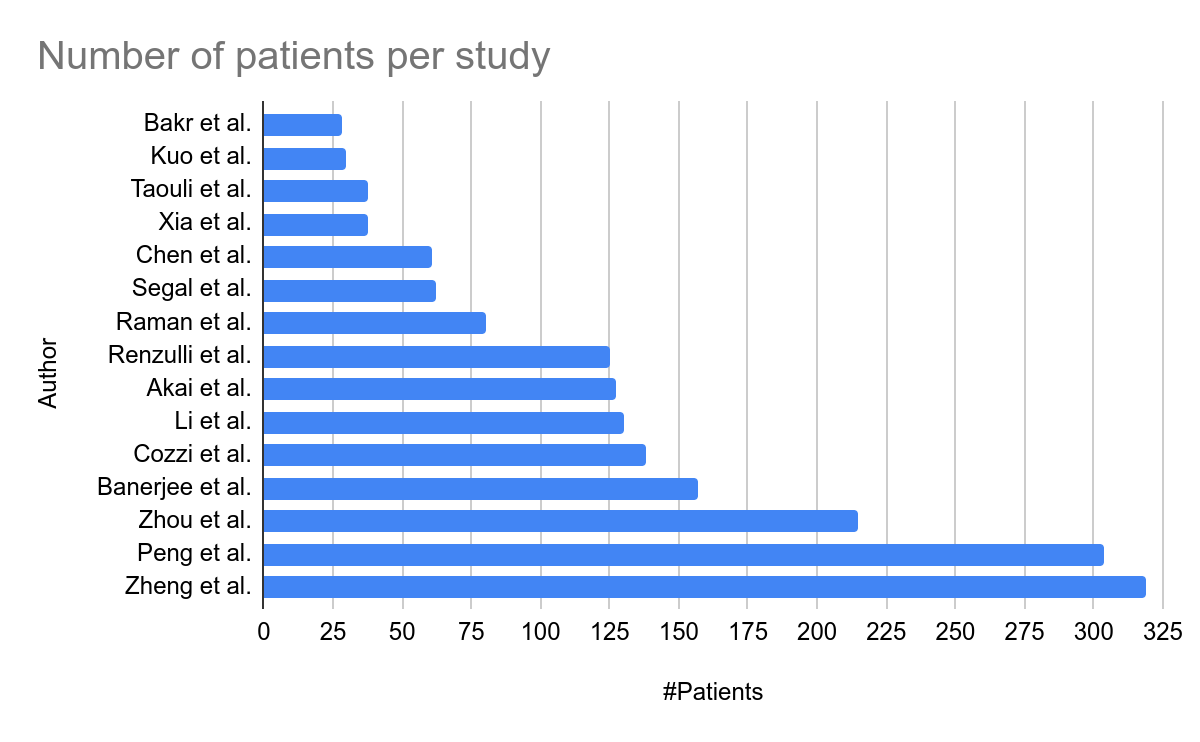
\includegraphics[width=0.7\linewidth]{images/image2}
	\caption{Number of patients included in the reviewed \ac{hcr} studies}
	\label{HCR_studies_number_of_patients}
\end{figure}



The relatively low number of patients can be explained by the stringent
inclusion criteria set by the studies (size and number of lesions,
baseline imaging examination within a given period of time before
initial treatment, \ldots{})\\
They were all built with data from patients who underwent CT
examination, except one, that decided to mix data obtained from both CT
and MR examinations \cite{Taouli2017}.

Regarding the CT scan protocol, only one study decided to use images
acquired before the injection of contrast agent \cite{Cozzi2017}, whereas two other studies used images acquired at only one
phase (early arterial phase for \cite{Raman2015}, and portal
venous phase for \cite{Li2016}), and the remaining studies
analyzed multiphase images. Among them, four studies utilized images
acquired at both early arterial and portal venous phases \cite{Zhou2017a,Chen2017,Kuo2007,Zheng2018}, while the rest were
based on traditional triphasic images \cite{Akai2018,Banerjee2015,Renzulli2016,Segal2007,Peng2018,Bakr2017,Taouli2017,Xia2018}. Concerning the
acquisition protocols, early arterial phase images are most of the time
acquired around 30s after the injection of contrast agent (between 22
and 35s), and some studies used bolus tracking method to estimate the
best acquisition moment instead of using the same timing for all the
patients. Portal venous phase images are acquired between 45 and 70s
after the injection, and the delayed images obtained during an even
larger interval (between 90 and 300s after the injection).\\
Knowing that images are the key elements in the computation process of
the radiomics features, this high variation within the acquisition
protocols is the first reason why the standard \ac{hcr} pipeline
should be standardized.

Once the images acquired, the following step consists in selecting the
region of interest to compute the features, or evaluate the
physiological properties of the lesions to the naked eye.

\subsubsection{ROI selection and features extraction}\label{roi-selection}

The selection of the region/volume of interest and/or the assessment of
the physiological characteristics of the tumor is often performed by one
or multiple experienced radiologists.
This step of the pipeline was performed by only a single expert in rare
cases in the reviewed studies \cite{Xia2018,Akai2018}, whereas it was
usually performed by two experts \cite{Zhou2017a,Chen2017,Li2016,Raman2015,Kuo2007,Renzulli2016,Segal2007,Zheng2018,Peng2018,Taouli2017}.
When more than one expert is involved, the authors decided to implement
ways for quantifying the inter and intra-observer variability, such as
the ICC (\emph{Intraclass Correlations Coefficient}) \cite{Zheng2018,Li2016}, or the Cohen-k statistics \cite{Renzulli2016,Banerjee2015}.
Regarding now the selection of the \ac{roi}, we can separate the reviewed
studies by the type of features being extracted.
On one hand, when using imaging traits corresponding to visual inspection of the tumor characteristics, it is common to use the whole tumor to perform the evaluation. For example when evaluating the
vascular invasion, some features like the peritumoral enhancement need
to be estimated globally \cite{Renzulli2016,Banerjee2015,Segal2007,Kuo2007}.
On the other hand, when using computational features, the analysis can
be performed on the whole tumor or on a single slice. Some studies
decided to compute the features on the entire 3D \ac{roi}, as an example
 Cozzi et al. \cite{Cozzi2017} used the entire tumor independently on
the tissues present within it , Xia et al. \cite{Xia2018} decided to separate
areas based on their textural properties  as depicted in the figure \ref{XiaFig_subregions}, but the
analysis remains global. Other studies placed several \ac{roi}s all throughout
the tumor (3 \ac{roi}s for Bakr et al. and from 5 to 10 for
Raman et al.). However, the majority of the studies decided to
place the \ac{roi} at the largest cross-sectional area \cite{Li2016,Chen2017,Zhou2017a,Akai2018,Zheng2018}.

\begin{figure}[ht!]
\centering
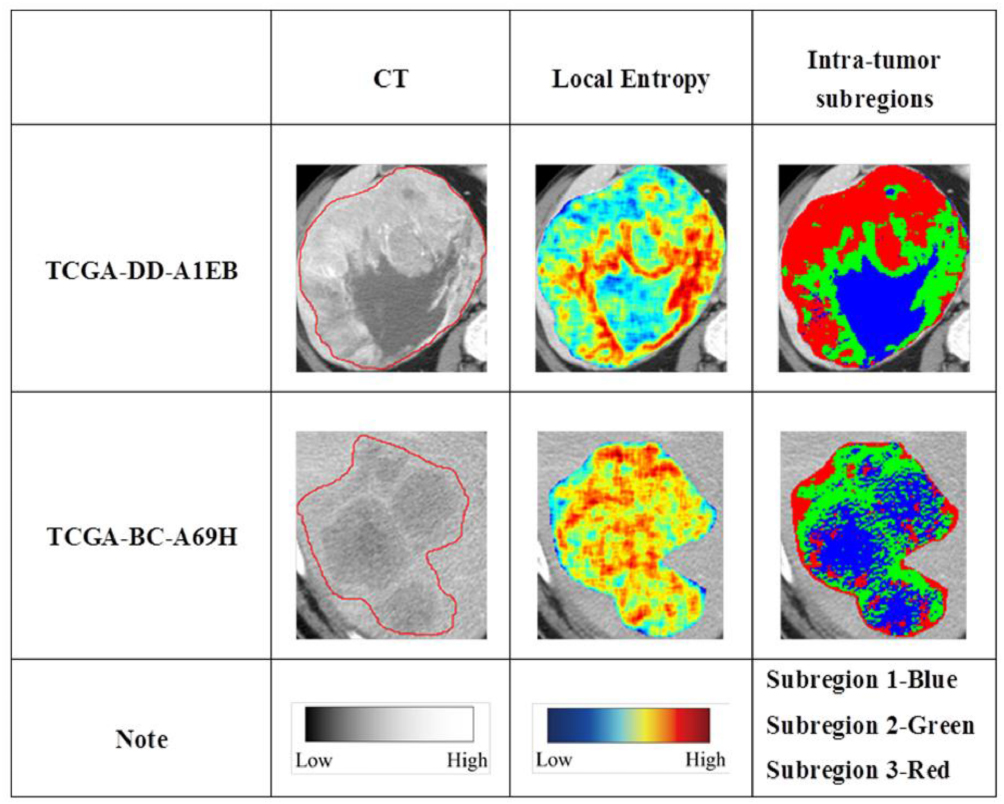
\includegraphics[width=4.34043in,height=3.46021in]{./images/image16.png}
\caption{Illustration of intratumor partition for two representative
patients (TCGA-DD-A1EB and TCGA-BC-A69H). The first column shows the
tumor outlines on the original CT image. The second column shows the
heatmaps of calculated local entropy on tumor images. The third column
shows the three subregions marked with different colors after intratumor
partitioning. \textbf{©Xia et al.} \cite{Xia2018}}
\label{XiaFig_subregions}
\end{figure}

Note that some studies decided to compute the features using both the
entire volume and the slice-wise approach (e.g. Taouli et al. \cite{Taouli2017}
evaluated imaging traits globally and computed the ratio using a
slice-wise fashion, Peng et al. \cite{Peng2018} did the same in their study by
computing features using an \ac{roi} placed at the largest-cross sectional
area, and evaluating imaging traits globally).\\
Worth mentioning that before the computation of features, it is common
to filter the images using different kernel sizes, in order to enhance
different elements of the volumes such as the blood vessels for example.
All reviewed studies that computed quantitative features filtered their
images with a Laplacian of Gaussian algorithm to extract features of specific sizes, as
depicted in the figure \ref{AkaiFig_Roi}.

\begin{figure}[ht!]
\centering
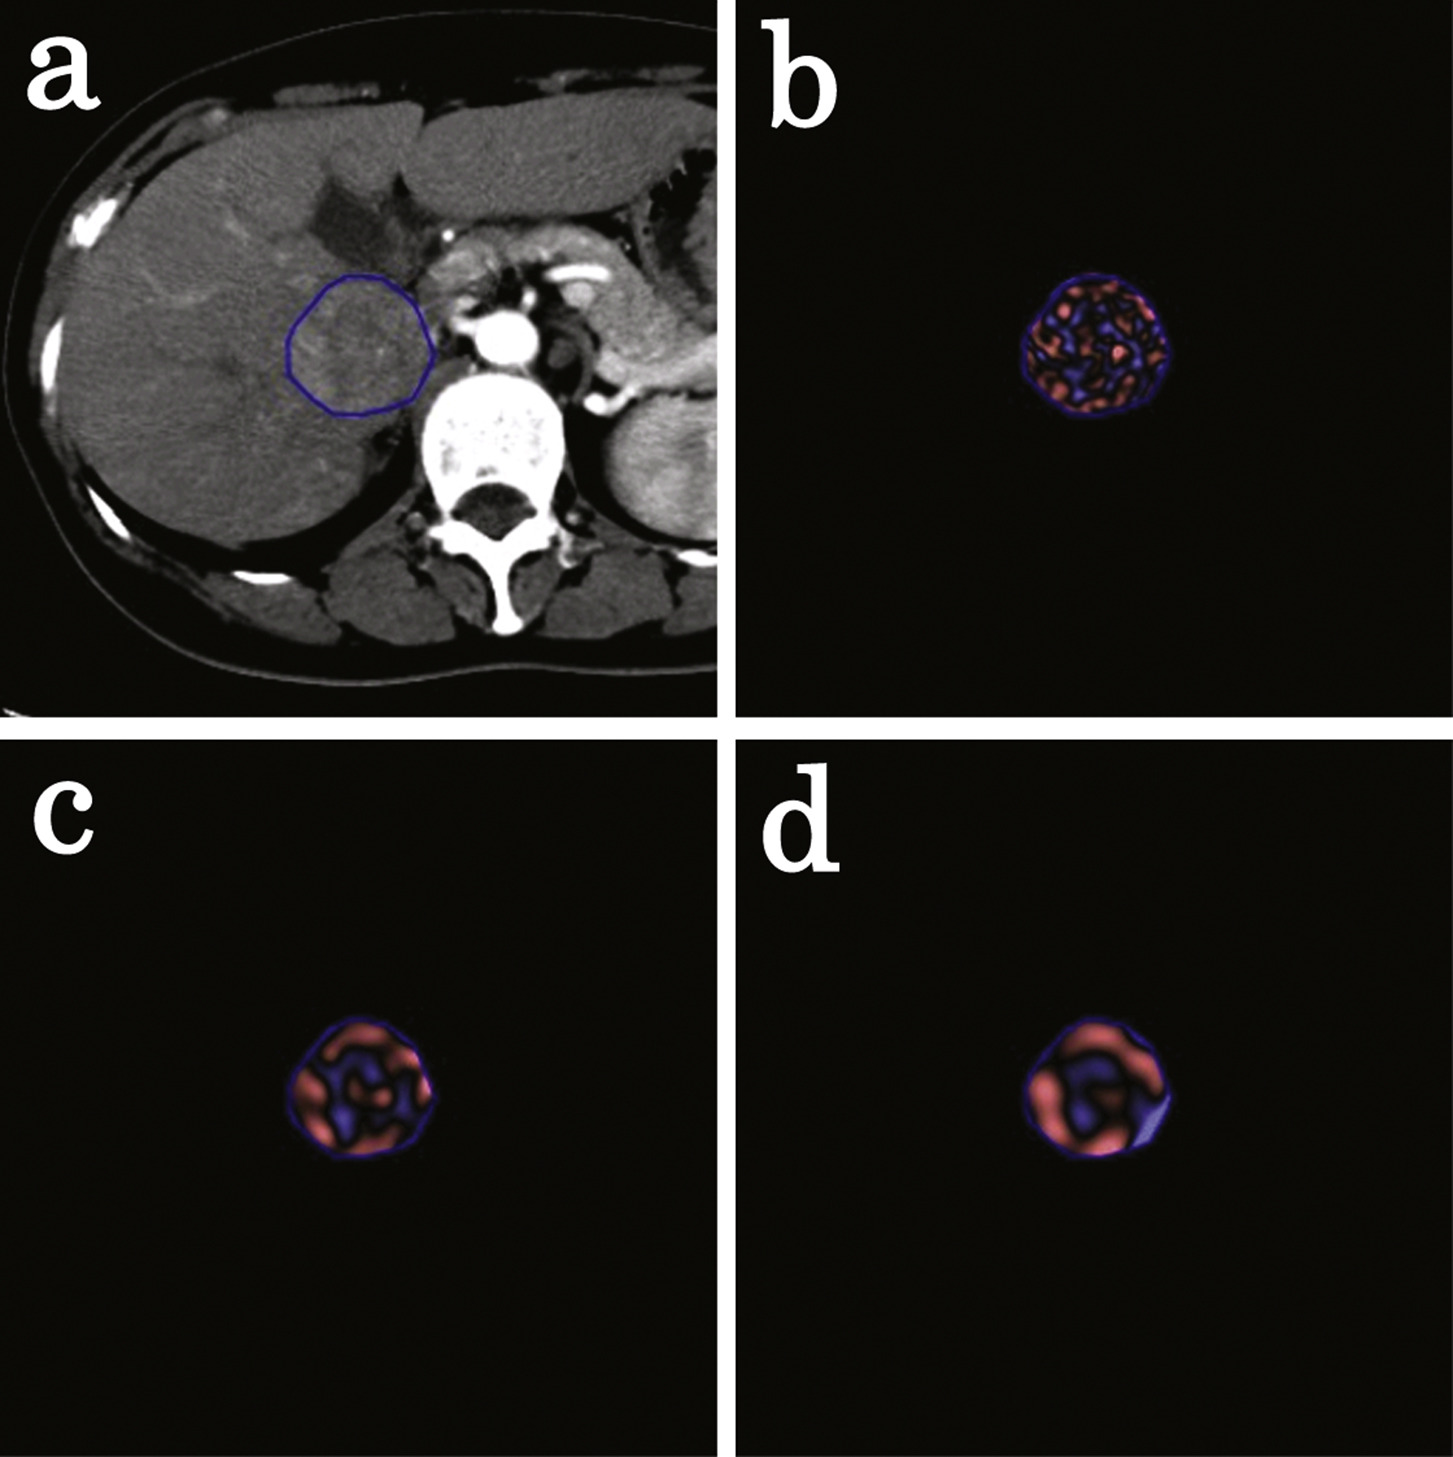
\includegraphics[width=3.50110in,height=3.51334in]{./images/image15.png}
\caption{ Screenshot of the CT texture analysis software. A polygonal \ac{roi} was
drawn on the tumor (a). Processed images using Laplacian of Gaussian
filters with SSF of 2 mm (b), 4 mm (c), and 6 mm (d) were automatically
generated. The images were displayed using a red or blue scale showing
negative or positive pixels, respectively. \textbf{©Akai et al.} \cite{Akai2018}}
\label{AkaiFig_Roi}
\end{figure}

\subsubsection{Features selection}\label{features-selection-1}

Once the \ac{roi} delineated and pre-processed, the following step consists
in extracting the features, and as explained previously, the choice on
which features to extract depends on the type of features the study is
going to rely on, quantitative or semantic.

In the case of quantitative features, the reviewed studies often decided
to focus on a single category of features (first-order, textural
features, higher-order\ldots{}), thus obtaining a relative small number
of features (27 for Li et al.\cite{Li2016}, 32 for Raman et al.\cite{Raman2015}).
However, despite choosing a specific category of features, this number
can increase, when combining the native features with the spatial
filter, and the different contrast enhanced phases, as in Akai
et al. where a total of 96 features are extracted from the initial 6
histogram-based features \cite{Akai2018}.\\
Some other studies decided to extract the maximum number of possible features by
combining the previously mentioned group of features, and thus obtained
300+ features \cite{Zhou2017a,Peng2018,Bakr2017}. The problem in this case, often called ``\emph{curse of
dimensionality}'', corresponds to a high number of features relative to
the number of individuals, and that can cause some troubles when further
training the predictable model. \\
When imaging traits are preferred to classical radiomics features, the
number of extracted characteristics is generally below 10, with a high
predominance of changes brought by the hepatocarcinogenesis, such as the
presence of internal arteries, or the wash-in wash-out effect (example
of imaging traits can be observed in the figure \ref{Segal_imagingTraits} \& \ref{Taouli_imagingTraits}). Even though
the number of extracted features is often small, they often correspond
to the absence or presence of physiological properties that are sometimes
difficult to quantify and that will highly depend on the observer
experience.

\begin{figure}[ht!]
\centering
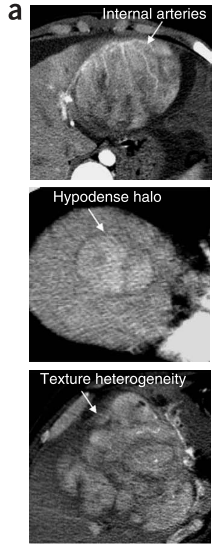
\includegraphics[width=1.13125in,height=2.82813in]{./images/image3.png}
\caption{From top to bottom: Internal arteries, Hypodense halo, Textural heterogeneity, as illustrated by \textbf{©Segal et al.} \cite{Segal2007}}
\label{Segal_imagingTraits}
\end{figure}

\begin{figure}[ht!]
\centering
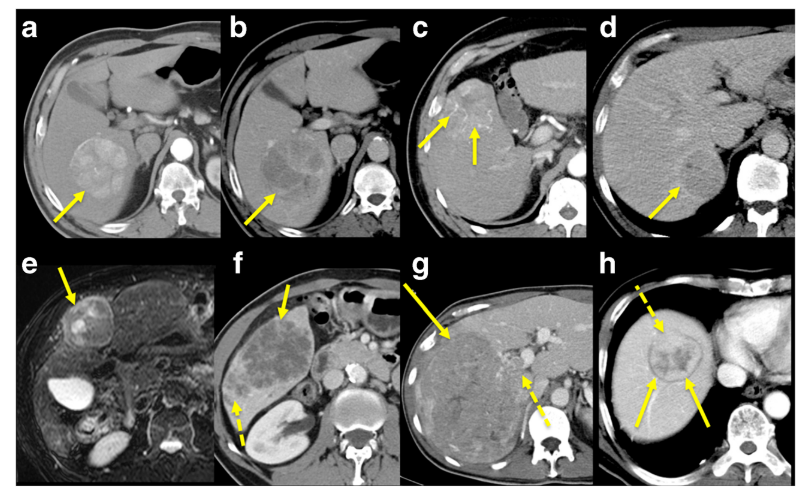
\includegraphics[width=4.67498in,height=2.86979in]{./images/image8.png}
\caption{
(a,b) wash-in/wash-out pattern and mosaic appearance, without capsule/
pseudocapsule.
(c) internal arteries (arrows)
(d) pseudo-capsule (arrow)
(e) {[}MR image{]} hyperintense encapsulated with mosaic appearance
(arrow)
(f) internal necrosis and satellite lesions posteriorly (dashed arrow)
(g) right portal vein invasion (dashed arrow)
(h) extra-nodular growth anteriorly (dashed arrow)
\textbf{©Taouli et al.} \cite{Taouli2017}
}
\label{Taouli_imagingTraits}
\end{figure}


After the different features are obtained, the next step in the pipeline
consists in the selection of the features and the building of the
predictive model.

The vast majority of the reviewed studies decided to implement a
logistical regression model in order to assess the correlation between
features and the study endpoint. Among the existing methods,
time-related approaches such as the Cox regression model \cite{Li2016,Banerjee2015,Zheng2018,Cozzi2017,Xia2018} and the Kaplan-Meier survival analysis
\cite{Segal2007,Chen2017,Akai2018,Xia2018} are the most commonly used.

Different statistical approaches were used by the studies that tried to
determine the link between selected features and study endpoints such as
the LASSO (\emph{Least Absolute Shrinkage and Selection Operator})
algorithm \cite{Zhou2017a,Peng2018,Bakr2017}. In the other studies, other
approaches were implemented, for example, Raman et al.
performed a \ac{pca} followed by a
MANOVA (\emph{Multivariate Analysis Of VAriances}) to create clusters
among patients for the classification of hypervascular lesions, whereas
Renzulli et al. evaluated the positive and negative predictive
values of the selected features against the microvascular invasion
status of the patients.
The list of discriminant features per study is given in the tables \ref{tab:QuantitativeFeatures}
 \& \ref{tab:SemanticFeatures} , with a separation between quantitative and semantic features.

\renewcommand{\arraystretch}{1}
\renewcommand{\baselinestretch}{1}

\begin{minipage}{17cm}
\begin{threeparttable} 
\caption{List of quantitative features used in the reviewed studies}
\label{tab:QuantitativeFeatures}
\begin{tabularx}{8cm}{|X|}
\hline
\emph{First Order Statistics}
\begin{itemize}
\itemsep0em 
\item Shape \cite{Cozzi2017}
\item Skewness \cite{Akai2018,Li2016,Zhou2017a}
\item Kurtosis \cite{Akai2018}
\item Mean \cite{Zhou2017a,Raman2015,Cozzi2017}
\item Energy \cite{Zhou2017a,Cozzi2017}
\item Entropy \cite{Peng2018,Akai2018}
\item Peak \cite{Bakr2017}
\item Standard deviation \cite{Xia2018}
\item Enhancement ratio \cite{Taouli2017}
\item Tumor-Liver difference \cite{Taouli2017}
\end{itemize}\\
\hline
\emph{Second Order Statistics} 
\begin{itemize}
\item Gray Level matrices \cite{Peng2018,Zheng2018,Cozzi2017}
\item Cluster prominence \cite{Xia2018}
\end{itemize}\\ \hline
\emph{Higher Order Statistics}
\begin{itemize}
\item Wavelets \cite{Chen2017,Li2016,Bakr2017}
\item Gabor \cite{Chen2017,Bakr2017}
\end{itemize}\\
\hline
\emph{Morphological features}
\begin{itemize}
\item Tumor margin volume \cite{Xia2018}
\item Tumor size\tnote{1} \cite{Renzulli2016,Taouli2017}
\end{itemize}\\
\hline
\end{tabularx}
\begin{tablenotes}
\item[1] {Not as an exact value, but classified (for example
the categories were smaller than 2 cm, between 2 and 5 cm, and larger than 5 cm in \cite{Renzulli2016})\par} 
\end{tablenotes}
\end{threeparttable}
\hspace{0.5cm}
\begin{threeparttable}
\caption{List of semantic features used in the reviewed studies}
\label{tab:SemanticFeatures}
\begin{tabularx}{7.5cm}{|X|}
\hline
\emph{Two Traits Predictor of Venous Invasion}
\begin{itemize}
\item Internal arteries \cite{Renzulli2016,Kuo2007,Peng2018,Segal2007,Banerjee2015,Taouli2017}
\item Hypoattenuating halos \cite{Renzulli2016,Peng2018,Segal2007,Banerjee2015}
\end{itemize} \\ \hline
\emph{Intensity-related features}
\begin{itemize}
\item Peritumoral enhancement \cite{Renzulli2016}
\item Presence of a Tumor-Liver difference \cite{Banerjee2015}
\end{itemize} \\ \hline
\emph{Textural-related features}
\begin{itemize}
\item Non-smooth Tumor Margins \cite{Renzulli2016,Kuo2007,Peng2018}
\item Infiltrative patterns \cite{Taouli2017}
\item Mosaic appearance \cite{Taouli2017}
\end{itemize} \\
\hline
\end{tabularx}
\end{threeparttable}
\end{minipage}


\renewcommand{\arraystretch}{5}
\renewcommand{\baselinestretch}{1.75}

\vspace{0.3cm}

Concerning the studies based on quantitative features we can notice that
first-order statistical features is the most common discriminant type,
which is normal because this group of histogram-based characteristics is
often implemented in the existing radiomics tools, whereas higher order
statistical features require more advanced knowledge to be implemented,
and often lack of interpretability. \\
Even though Li et al. \cite{Li2016} decided to extract only Wavelet features
because they consider that the current way of computing textural
features is too dependent on the imaging acquisition settings, first and
second-order statistical features remain a good indicator of the
textural heterogeneity which is often correlated with the physiological
advances of the disease.\\
Worth also noting that imaging traits, often analyzed either alone, or
in combination with quantitative features, remain discriminant enough in
a lot of studies, because they are directly linked to the physiological
changes produced by the disease. Despite needing expertise to be
extracted, such as in Segal et al. where 32 different imaging
traits were analyzed, their predictable power drives us to consider them
in future radiomics studies and focus on a way to quantify them \cite{Segal2007}.

\subsubsection{Study reproducibility}\label{study-reproducibility}

Although the majority of the reviewed studies obtained good predictable
results in regards with the wanted prediction task, their stability to
the experimental settings and their reproducibility remain questionable.

In 2017, Lambin et al. \cite{Lambin2017} who remains one of the founders of the
radiomics fields \cite{Lambin2012} published a study
proposing a way to rethink the \ac{hcr} pipeline and assess the reproducibility of
future radiomics studies . This
assessment is performed thanks to the RQS (\emph{Radiomics Quality
Score}), which evaluates a total of 16 components with various weights.
The evaluation of the different components allows the computation of a
score ranging from 0 to 36 points where highest weights are given to
criteria allowing a better reproducibility of the study, such as the
prospective aspect of the study (7 points over 36) or the presence of a
validation step in the proposed workflow (5 points over 36, with a
penalty of 5 points when no validation at all is present). \\
Our reviewed studies were evaluated in regards with the RQS, in
consensus with a medical research fellow (Wakabayashi Taïga) \cite{Wakabayashi2019}.
The details of the different scores per study are reported in the table \ref{tab:RQS_details}.


\renewcommand{\arraystretch}{1}
\setlength{\tabcolsep}{7pt}
\newgeometry{top=5mm, left=5mm, right=5mm, bottom=10mm, footskip=5mm, headsep=10mm}
\begin{landscape}
\scriptsize
\centering
\mbox{}\vfill
\begin{table}[!htp]
\caption{RQS score details per criteria for the reviewed studies}\label{tab:RQS_details}
\scriptsize
\begin{tabular}{p{3.8cm}|p{1cm}p{1cm}p{1cm}p{1cm}p{1cm}p{1cm}p{1cm}p{1cm}p{1cm}p{1cm}p{1cm}p{1cm}p{1cm}p{1cm}p{1cm}p{1cm}p{1cm}p{1cm}}\toprule
\textbf{Criteria} &\textbf{Bakr et al.\cite{Bakr2017}} &\textbf{Kuo et al.\cite{Kuo2007}} &\textbf{Taouli et al.\cite{Taouli2017}} &\textbf{Xia et al.\cite{Xia2018}} &\textbf{Chen et al.\cite{Chen2017}} &\textbf{Segal et al.\cite{Segal2007}} &\textbf{Raman et al.\cite{Raman2015}} &\textbf{Renzulli et al.\cite{Renzulli2016}} &\textbf{Akai et al.\cite{Akai2018}} &\textbf{Li et al.\cite{Li2016}} &\textbf{Cozzi et al.\cite{Cozzi2017}} &\textbf{Banerjee et al.\cite{Banerjee2015}} &\textbf{Zhou et al.\cite{Zhou2017a}} &\textbf{Peng et al.\cite{Peng2018}} &\textbf{Zheng et al.\cite{Zheng2018}} \\\toprule
\textbf{Image Protocol quality} &1 &2 &2 &2 &2 &1 &2 &2 &2 &2 &1 &2 &2 &2 &2 \\
\textbf{Multiple segmentations} &1 &0 &0 &0 &1 &1 &1 &0 &0 &1 &0 &1 &1 &1 &1 \\
\textbf{Phantom Studies} &0 &0 &0 &0 &0 &0 &0 &0 &0 &0 &0 &0 &1 &0 &0 \\
\textbf{Multiple time points} &0 &0 &0 &0 &0 &0 &0 &0 &0 &0 &0 &0 &0 &0 &0 \\
\textbf{Features reduction} &-3 &3 &3 &3 &3 &3 &-3 &3 &3 &3 &3 &3 &3 &3 &3 \\
\textbf{Mutlivariate analysis} &1 &1 &1 &1 &1 &0 &0 &0 &1 &1 &1 &1 &1 &1 &1 \\
\textbf{Biological correlates} &0 &1 &1 &1 &0 &1 &0 &0 &0 &0 &0 &1 &0 &0 &0 \\
\textbf{Cut-off analysis} &0 &0 &0 &0 &1 &1 &1 &0 &1 &1 &1 &0 &1 &1 &1 \\
\textbf{Discrimination statistics} &2 &1 &0 &0 &1 &1 &1 &1 &2 &1 &1 &1 &1 &1 &1 \\
\textbf{Calibration Statistics} &0 &0 &1 &2 &0 &1 &0 &0 &1 &1 &1 &1 &0 &2 &1 \\
\textbf{Prospective study} &0 &0 &0 &0 &0 &0 &0 &0 &0 &0 &0 &0 &0 &0 &0 \\
\textbf{Validation} &-5 &-5 &-5 &-5 &-5 &3 &-5 &-5 &-5 &-5 &-5 &5 &-5 &2 &2 \\
\textbf{Gold standard comparison} &2 &2 &2 &2 &0 &0 &2 &0 &2 &0 &2 &2 &2 &2 &2 \\
\textbf{Clinical utility} &2 &2 &2 &2 &2 &2 &2 &2 &2 &2 &0 &2 &2 &2 &2 \\
\textbf{Cost-effectiveness analysis} &0 &0 &0 &0 &0 &0 &0 &0 &0 &0 &0 &0 &0 &0 &0 \\
\textbf{Open science Data} &0 &0 &0 &0 &0 &1 &0 &0 &0 &0 &0 &0 &0 &0 &1 \\
\bottomrule
\textbf{Total} &\textbf{1} &\textbf{7} &\textbf{7} &\textbf{8} &\textbf{6} &\textbf{15} &\textbf{1} &\textbf{3} &\textbf{9} &\textbf{7} &\textbf{5} &\textbf{19} &\textbf{9} &\textbf{17} &\textbf{17} \\
\bottomrule
\end{tabular}
\end{table}
\vfill
\end{landscape}
\renewcommand{\arraystretch}{5}
\newgeometry{vmargin={15mm}, hmargin={30mm,30mm}}   % set the margins 


The mean obtained \ac{rqs} by the reviewed studies was 8.73 $\pm$ 5.57
points, which corresponds to less than 23\% of the maximal possible
score, and only one study obtained a more than 50\% of the maximum
points, which translates the lack of robustness of the current
\ac{hcr} state-of-the-art studies applied to the HCC.

The figure \ref{RQS_points_per_criteria} allows us to see the most respected criteria in regards
with the RQS guidelines.


\begin{figure}[th!]
\centering
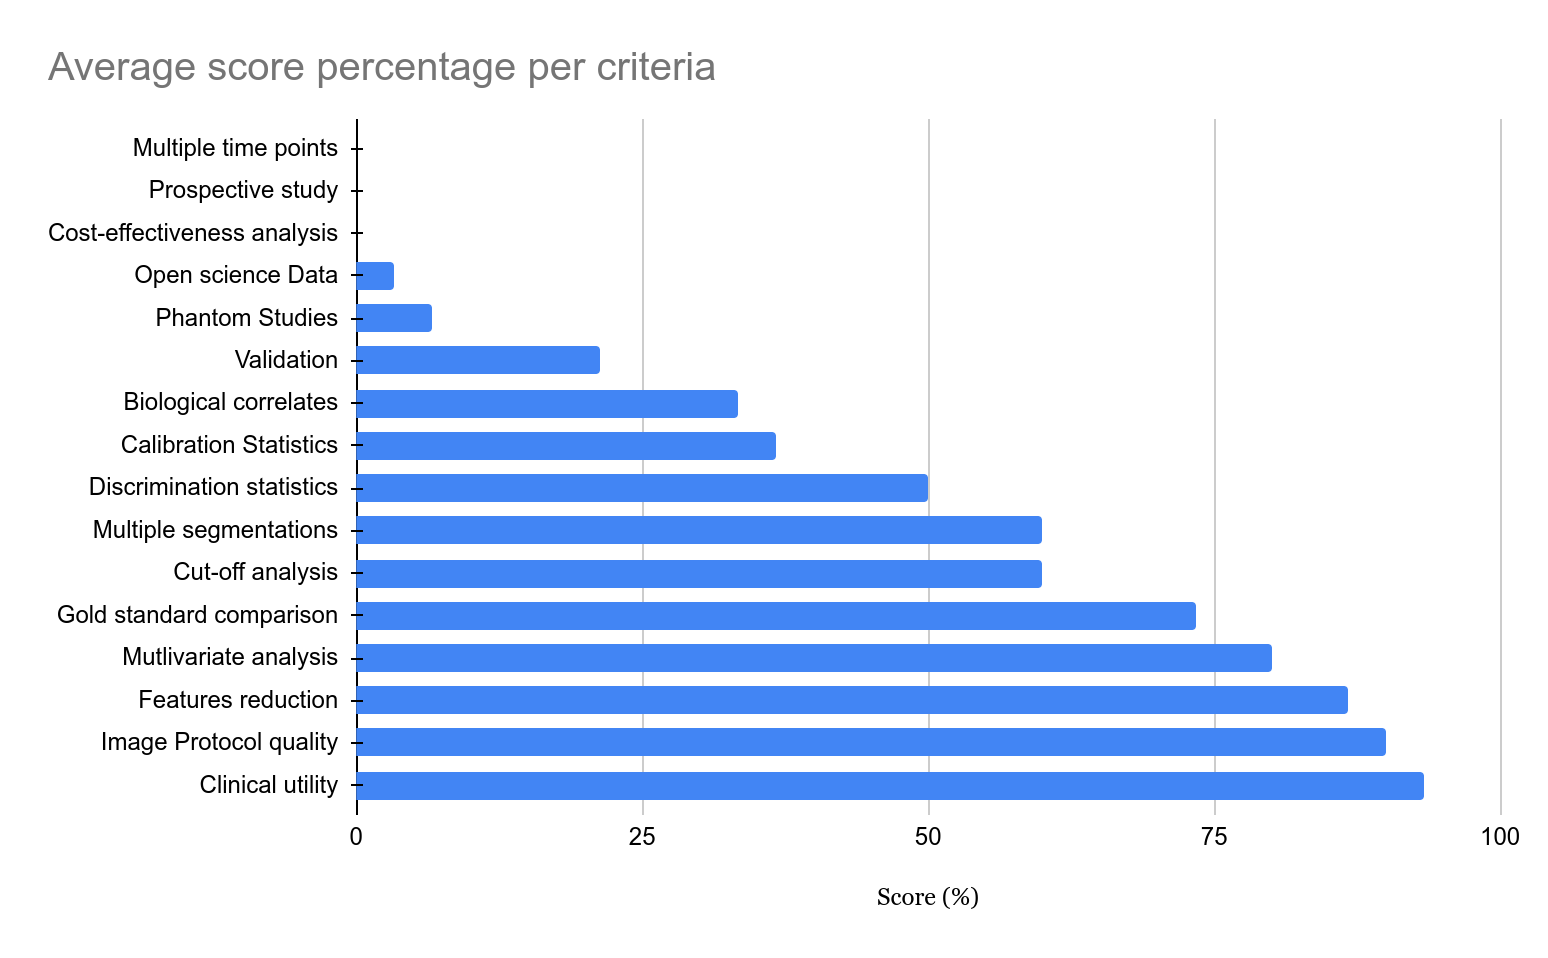
\includegraphics[width=0.7\linewidth]{images/image13}
\caption{Average score percentage per criteria in the \ac{rqs} for the reviewed studies}
\label{RQS_points_per_criteria}
\end{figure}


The criteria the less respected by the different reviewed studies were
all those related with the reproducibility and the robustness. Among
them, the analysis of images acquired at multiple times, the
implementation of phantom studies to detect inter-scanner differences
and features sensitive to those settings, or even the prospective design
of the studies that will ensure inclusion of patients undergoing the
same protocols were almost always neglected.
Even though the different reviewed studies obtained successful results
in regards with the wanted task, their robustness relative to the
experimental settings and their reproducibility can be questioned,
especially when analyzing their results obtained on the radiomics
quality scoring system \cite{Lambin2017}. \\
One way to allow a better reproducibility for the future radiomics
studies is to fulfill the maximum possible criteria introduced by the
RQS standard, and to use standard ways to compute the
quantitative features, thanks to open-source libraries such as
pyradiomics \cite{VanGriethuysen2017}. Another way is to reduce as much
as possible the impact of human-based interpretation in the \ac{hcr}
workflow. This can be done by replacing the hand-crafted annotations,
and the engineered process of features computation and selection by a
standardized, automated and data-driven pipeline, similar to what is
performed in more recent \ac{dlr} studies.

\section{Deep Learning Radiomics}\label{deep-learning-radiomics}

In this section we will first present the value brought by the deep learning in the medical imaging field, before focusing on the differences between the
\ac{hcr} and the \ac{dlr} strategies. We will then describe in detail
the \ac{dlr} concept before presenting the different reviewed
studies tackling liver-related problems using a \ac{dlr} approach. We
will outline the different steps of their pipelines such as the use of
multiphasic images, the way they incorporated experts' annotations and
their choice regarding the deep network architectures.

\subsection{\ac{dl} applied to the medical imaging}

The main breakthrough brought by \ac{dl} was its ability to detect
morphological properties in images only by using the pixel intensities
as input, whereas traditional machine learning methods often required
sophisticated hand-crafted features to achieve descent results \cite{Litjens2017, Suzuki2017}. Deep learning networks achieved
state-of-the-art results in many medical-related applications among
which classification, localization, detection, registration and
segmentation \cite{Ker2017}. Even with a small number of
training cases, those performances were realized thanks to architecture
choice, data augmentation or transfer learning \cite{Zheng2018, Hu2018}.
As exposed previously, the automatic segmentation of the tumors brings a
volumetric information, that is more powerful than the diameter only,
and that allows to compute the tumor burden, which has an importance
when estimating the efficiency of a given treatment \cite{Gobbi2004, Bornemann2007, Heussel2007, Kuhnigk2006, Puesken2010, Bauknecht2010}.\\

\subsection{DLR to tackle HCR limitations}\label{difference-between-hcr-and-dlr}

Being a recent field, radiomics starts to mature when applied to several
organs such as the lungs or the breast, but it still struggles when
applied to the liver, especially because of the scarcity of available
data and the complexity of its anatomy.
As exposed previously, the first studies targeting liver cancer almost
always rely on hand crafted features.
The main limitation observed is the lack of reproducibility originating
from engineered features, that sometimes result from complex processes
which can be difficult to imitate, and often fail to work on different
databases. \ac{hcr} often rely on manual or semi-automatic expert annotations, which
often require a complex and time-consuming process, that also provide
several constraints, such as the poor inter-expert reproducibility.
The extracted features are not necessarily relevant to encode the
observed structure, it is needed to increase their number, hence
requiring a complex dimensionality reduction step.
Another limitation is the difficulty to find the perfect association
between features extraction, selection and the statistical analysis used
to reach the wanted target.\\
Those limitations, and the rise of new computational resources
associated with the emergence of deep learning techniques allowed the
development of a new branch in the radiomics field, called \ac{dlr}
(Deep-Learning Radiomics) \cite{Afshar2018}.

\subsection{DLR workflow}\label{dlr-workflow}

In this branch of radiomics, the features are extracted through a
deep-learning process, avoiding a manual extraction.
A neural network can be trained to generate the most relevant features.
These features can either be kept in the network for the final
pathological target prediction, or used as input in a different model
(such as a \ac{svm} or a RF).
Compared to the \ac{hcr}, less prior knowledge is required, and the
features can be extracted in an end-to-end manner, using only the raw
images as input, and without necessarily providing any segmentation. It
has also been demonstrated that performances of those networks increase
with the size of the training dataset \cite{Cheng2016}.
Eliminating the segmentation phase when evaluating the diagnosis, allows
to reduce the workload of experts, and provides a solution to the
observer-dependency.
When training \ac{dlr} networks, the original image can be combined
with the segmentation or any other pre-processed step result such as the
gradient image for example \cite{Sun2017a} to improve
the relevance of the extracted features.

Generally, \ac{dlr} studies can be classified depending on the type of
input used, the training strategy or the type of architecture chosen to
extract the features.\\
As input, deep radiomics networks can consider 2D slices independently,
however this technique does not bring sufficient information since the
decision mainly depends on the entire volume of interest.
The different outputs obtained in a slice-wise fashion can be fused to
get a volume-wise decision. The volume by itself can also directly be
used as input, however it can raise several issues such as the size of
the voxels or the slice thickness. Finally, the classification can be
performed by considering a series of volumes corresponding to the entire
examination of the patient \cite{Shen2016}, but here
again the question regarding the normalization of the input can be
raised. \\
Once the type of input is chosen, the studies differ depending on the
type of network and the training strategy utilized. 
The networks can be trained \emph{from scratch} using
only the available data or a pre-trained architecture can be fine-tuned.
In the first case, the obtained network will be specific to the wanted
task, but this specialization can also lead to troubles such as
overfitting or the sensitivity to class imbalance.
The impact of those problematics can be limited with the help of data
augmentation (use of existing data to generate new artificial samples) \cite{Kumar2017}, multi-task training (where the
number of parameters is limited by the training of several task using
the same network) or the
incorporation of the proportion of each class present in the data when
building the cost function \cite{Jamaludin2016}.
The other strategy consists in using an architecture pre-trained most of
the time on natural images, and then re-train only a specific part 
using the desired dataset \cite{Echaniz2017,Huynh2016,Paul2016}. It
is worth noting that this type of training constrains the pipeline to be
slice-wise since existing architectures are often pre-trained on 2D
images.\\
Finally, the features can be extracted using either a supervised or an
unsupervised approach. In the supervised case, the most commonly used
networks are based on convolutional layers (CNN), followed by one
or multiple dense layers to predict the output class. While the network
is trained to perform the classification, the features are extracted
either after a fully connected layer \cite{Paul2016}, or after one 
of the convolutional layers \cite{Li2017}.\\
Other variants that are also built with convolutional layers as key
components can also be implemented (RNN: \emph{Recurrent Neural Networks}, LSTM: \emph{Long Short Term Memory} or
\emph{Capsule Net}). Their goal is to get rid of the limitations caused
by the input format that need to be fixed, and by the difficulty to
consider an entire 3D volume during the training \cite{Azizi2018}.
In the unsupervised case, the objective is to learn the data distribution,
so that new data from the same distribution can be generated. 
The most commonly used architecture
in this case is the \emph{auto-encoder}, made up with a part that
contracts the information (encoder), in order that the most useful one
is conserved to regenerate the original data (decoder). Auto-encoder can
be built on top of convolutional layers \cite{Echaniz2017}, 
or trained with the aim of being insensitive to the noise
added to the input data (\emph{denoising auto-encoder})\cite{Sun2017a,Kim2016}. 
Following the same principles which are to reconstruct the
original input data using only the most relevant features, some studies
implemented other type of generative models such as the 
DBN (\emph{Deep Belief Networks}) \cite{Sun2017a} or Deep Boltzmann Machines \cite{Suk2014}.

Some studies are referred to as hybrid, when features are combined with
other sources of data (combination of different modalities 
\cite{Oikonomou2018} or association with clinical
data such as genomic data \cite{Emaminejad2016}), or
when only a part of the pipeline implements deep learning methods,
either for the extraction of the features \cite{Paul2016} or when the decision is taken with a fusion between \ac{hcr}
and \ac{dlr} features \cite{Huynh2016}.

\subsection{\ac{dlr} applied to the liver}\label{dlr-applied-to-the-liver}

Even though the number of studies targeting the liver is increasing, the
vast majority of them can be categorized as \ac{hcr}, and only a few
are currently based on deep learning.
The main reason behind that is the late emergence of deep learning and
the recent outbreak of new architectures and concepts that are often
first developed and evaluated in other fields than the medical imaging
one (e.g. Residual Network, DenseNet, Capsule Net).\\
However, we have decided to review the first \ac{dlr}-liver related studies, in order to understand how \ac{dl} architectures can successfully be incorporated in a radiomics pipeline. We describe the study endpoints, the data preprocessing, the implementation and training strategies, before analyzing their performances. A more detailed analysis of the reviewed studies is available in the following \href{http://bit.ly/dlr_studies_summary}{link} \footnote{\url{http://bit.ly/dlr_studies_summary}}.

\subsubsection{Study Endpoint}\label{study-endpoint}

Within the reviewed \ac{dlr} studies, the majority of them are
targeting a characterization of the tumor, either the classification of \ac{fll}s (\emph{Focal
Liver Lesions}) \cite{Yamada2019,Wang2018,Yasaka2018,Liang2018}, the estimation of the fibrosis
stage \cite{Yasaka2018a}, or the prediction of the histological grade \cite{Yang2019} when two of them focused on the
response to treatments, either for recurrence after resection \cite{WANG2019} or the response after TACE (\emph{TransArterial ChemoEmbolization})\cite{Peng2020}.\\
We selected the studies using CT images to perform their
analysis, and realized that the vast majority of them used multiphasic
images to perform their research, knowing that the evolution of contrast
medium is often correlated with the pathological features of the liver
as mentioned in the chapter \ref{liverCancer}. The only one that used
single phase images, was the one targeting an estimation of the fibrosis
stage, and their method was based on portal phase images only \cite{Yasaka2018a}. 
Regarding the multiphasic studies,
there is no consensus about the delay between the injection of the
contrast agent and the acquisition of the different phases. They tend to
prefer triphasic acquisition, with images acquired before the injection
of contrast agent, at early arterial phase and a third phase, either
portal venous \cite{WANG2019,Wang2018,Liang2018} or a delayed one \cite{Yamada2019, Yasaka2018}. Peng et al. decided to get rid of the \ac{nect}
(\emph{Non-Enhanced CT}) phase, but still chose a triphasic acquisition
(\ac{ar}, \ac{pv}, DELAY).
The only retained study performing its analysis on MR images \cite{Yang2019}, also used multiphase images, were 5 phases were processed (precontrast, late arterial, portal venous, equilibrium and delayed phases).

\subsubsection{Image processing pipeline}\label{image-processing-pipeline}

Concerning the image processing pipeline, the data used to train the
deep networks are most commonly selected via placement of a bounding box
by the experts around the hepatic lesion \footnote{Although some parts of the pipeline are being processed by DL networks, it is worth noting that among the analyzed DLR-studies, the definition of the region of interests and the registration is still often manually performed, hence, highlighting current limitations of the first DLR-based studies.}, before a registration between
the different phases in case of multiphasic acquisition to compensate the
effects of body motion and/or breathing.\\
The manual delineation of the \emph{\ac{roi}s} is usually done by one or more
experts on the raw image \cite{Yamada2019,Wang2018,Yasaka2018a,Yasaka2018,WANG2019,Yang2019}, and only one study decided to perform an automatic segmentation of both the
parenchyma and the lesion with the application of a random-walker
algorithm, before being checked by experts \cite{Liang2018}. 
When the method is based on a 2D approach, selected images are
often those presenting the maximal cross-sectional proportion of the
lesions, except one study targeting the estimation of the fibrosis
stage, that centered the \ac{roi} so it displayed the ventral aspect
of the liver \cite{Yasaka2018a}. Only one study
incorporated 3D information in their pipeline, but they also started the
placement of the \ac{voi} with the slice presenting the maximal
proportion of tumor, and extended it to adjacent slices \cite{Yang2019}.\\
After placing a bounding box, the images are registered either manually \cite{Yamada2019,WANG2019,Wang2018} or
via the application of a non rigid registration with anatomical constraints \cite{Liang2018}. No real registration was mentioned for
two studies \cite{Peng2020,Yasaka2018a} but
Yamada et al. evaluated the effects of the registration in the
prediction performances of their networks (as depicted in the figure \ref{Yamada2019_Fig1}), 
and after training several networks with misregistered data
(shifted, rotated, skewed) they concluded that in the vast majority of
the cases, no statistical significance can be found between the
performances of the networks trained with manually registered data and
those of the networks trained with misregistered data \cite{Yamada2019}.


\begin{figure}[th!]
\centering
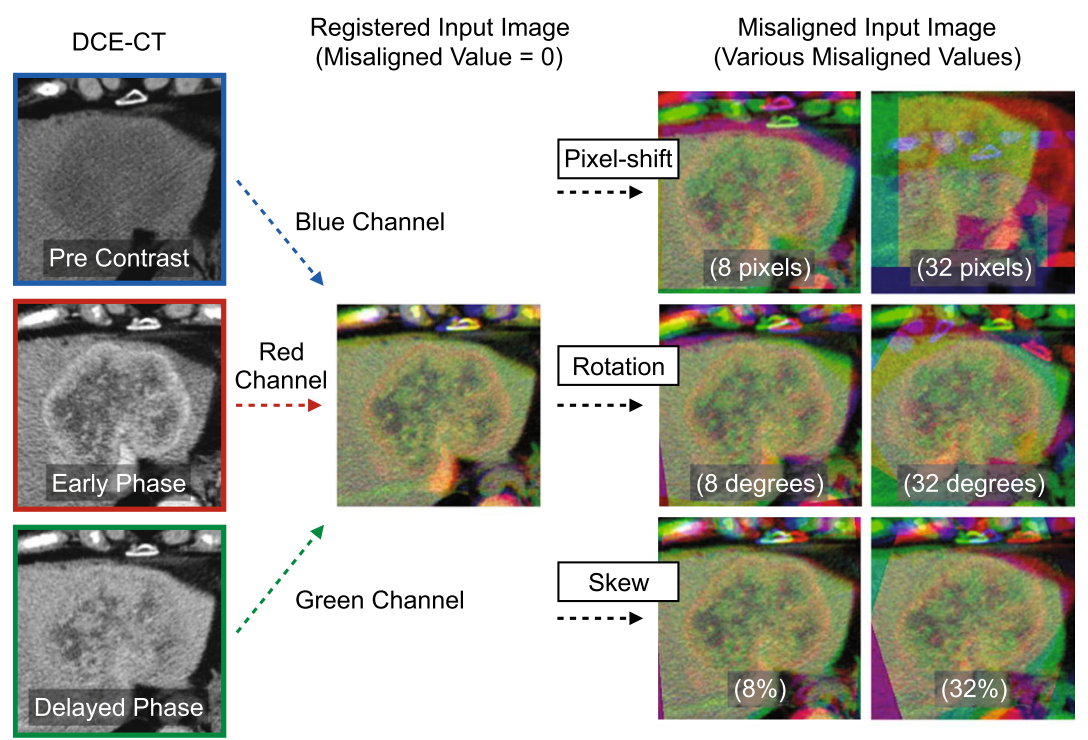
\includegraphics[width=0.7\linewidth]{images/image12}
\caption{Illustration of the manually registered images and the effect of transformations (shift, rotation, skew) in the three phases, by \textbf{©Yamada et el. \cite{Yamada2019}}}
\label{Yamada2019_Fig1}
\end{figure}


It is worth noting that some studies performed their analysis on cropped or
resized JPEG images \cite{Yasaka2018,Yasaka2018a,WANG2019}. 
This choice might cause loss of data whereas the raw images are used elsewhere with the native HU (\textit{Hounsfield Unit}) intensities.\\
Finally, in the reviewed studies, only two of them combined images with
clinical data \cite{Yasaka2018a,WANG2019}, whereas the other only used image data, which is
comprehensible because clinical data are often difficult to retrieve,
and can also be difficult to integrate in a deep network, as illustrated
in the figure \ref{Wang2019_Fig2}.
\begin{figure}[th!]
\centering
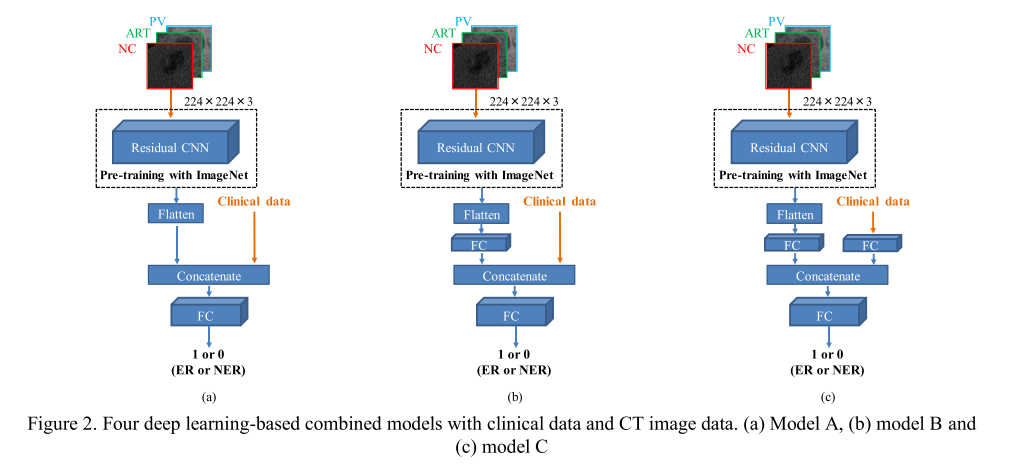
\includegraphics[width=1.0\linewidth]{images/image5}
\caption{Illustration given by \textbf{©Wang et al.} of the different tested deep networks where raw images are combined with the clinical data \cite{WANG2019}}
\label{Wang2019_Fig2}
\end{figure}


\subsubsection{Architecture choice}\label{architecure-choice}



The reviewed studies differ mainly in the way they built their deep
architecture.

In most of the cases, convolutional layers are used for the extraction
of the most discriminant features. The main question being whether to
use a pre-trained network or to train a network from scratch. In the
case of fine-tuning, the most commonly used architectures are the
AlexNet and the ResNet \cite{WANG2019,Wang2018,Yamada2019,Peng2020}, but it is also usual to
compare the results obtain by different pre-trained architectures \cite{WANG2019,Yamada2019}. The general method
is to recycle an architecture trained on a huge dataset such as
ImageNet, freeze the weights of the early layers (responsible for the
high levels features), adjust and train the last layers on the current
database to be more specific.
An illustration of this process can be found in the figure \ref{Wang2018_Fig3}.

\begin{figure}[th!]
\centering
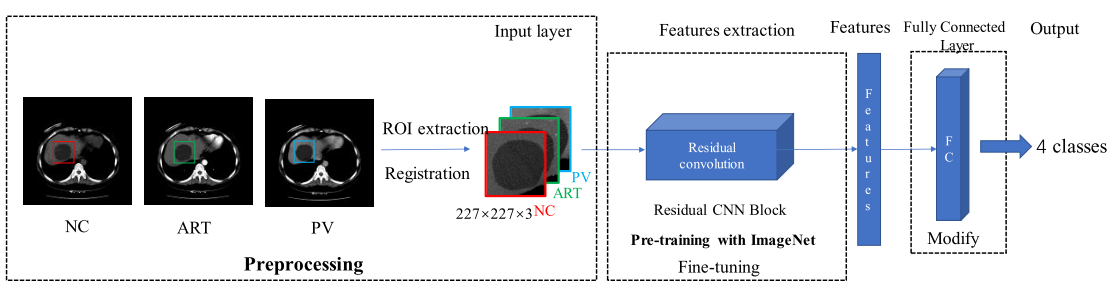
\includegraphics[width=0.9\linewidth]{images/image6_crop}
\caption{Illustration of the pre-training strategy adopted by \textbf{©Wang et al.} \cite{Wang2018}}
\label{Wang2018_Fig3}
\end{figure}


The rest of the reviewed studies created a custom architecture and
trained it from scratch \cite{Yasaka2018a,Yasaka2018,Liang2018,Yang2019}.
Two of them used classical convolutional layers followed by max pooling
layers, early in the network to extract relevant features, as depicted
in the figure \ref{Yasaka2018_Fig2}.

\begin{figure}[th!]
\centering
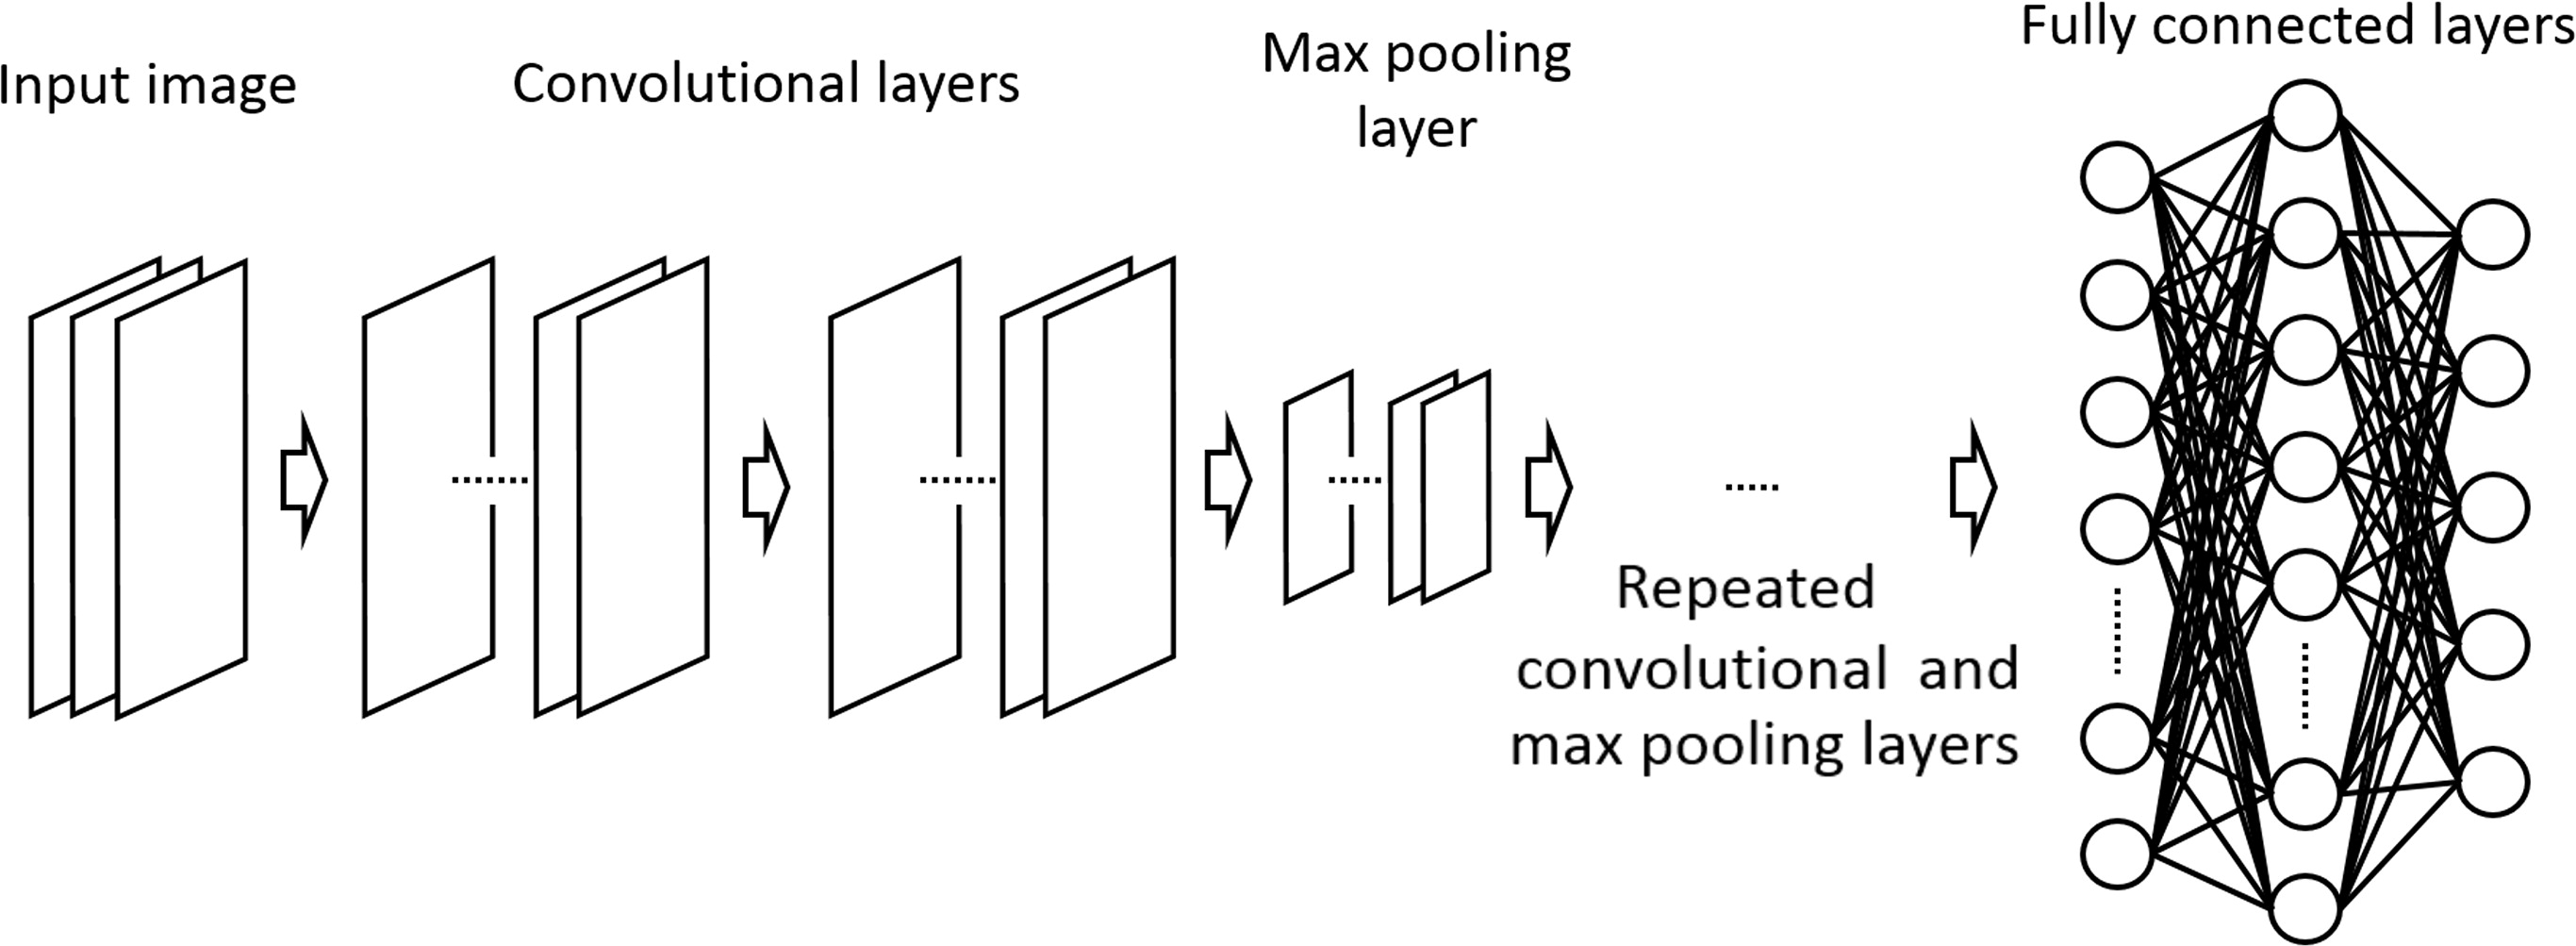
\includegraphics[width=0.7\linewidth]{images/yasaka2018}
\caption{Architecture used by \textbf{©Yasaka et al.} where the features are first extracted through convolutional layers before the prediction is performed using fully connected layers. \cite{Yasaka2018}}
\label{Yasaka2018_Fig2}
\end{figure}

Since multiphasic studies often stacked the different phases as channels
to feed the deep network, one study decided to extract the temporal
information through a different paradigm by using LSTM layers \cite{Liang2018}. As depicted
in the figure \ref{Liang2018_Fig1}, their architecture first extracted the features using what they
called a ``ResGLBlock'' per phase, with two scaled data as input (a
large one with the entire lesion, and a smaller one with finer details),
and conserved the temporal information via bidirectional LSTM
layers.

\begin{figure}[th!]
\centering
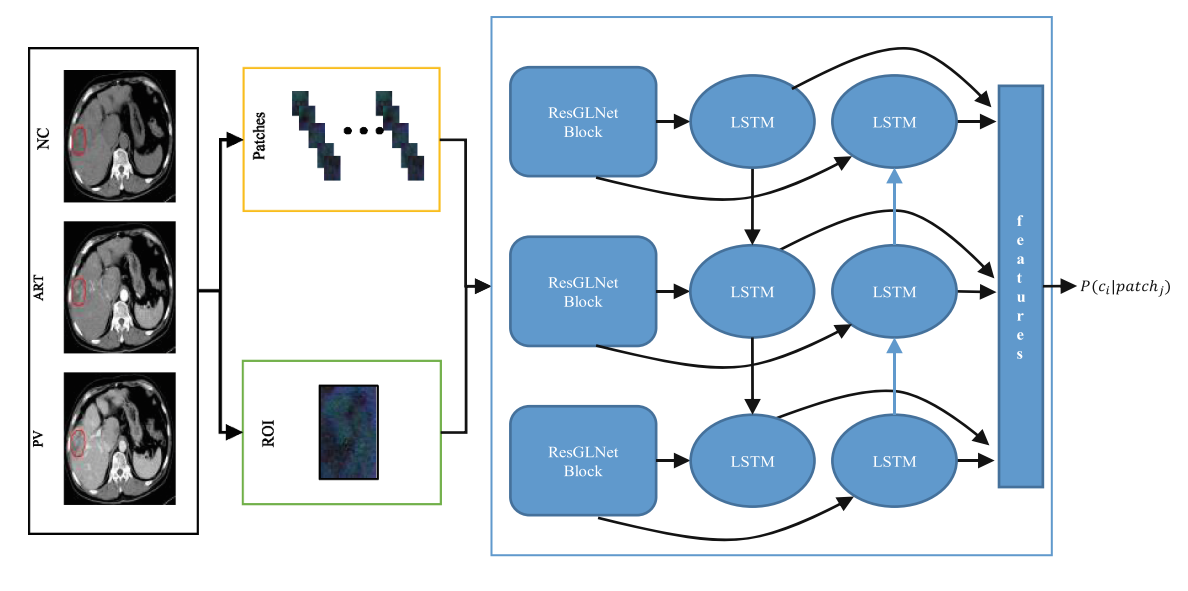
\includegraphics[width=0.7\linewidth]{images/image7_crop}
\caption{Architecture used by \textbf{©Liang et al.} where patches of different scales are extracted from the original images, before being used to train residual networks connected with bidirectional LSTM layers \cite{Liang2018}}
\label{Liang2018_Fig1}
\end{figure}

Yang et al also created a custom architecture to incorporate the dynamic information \cite{Yang2019}.
The used architecture is depicted in the figure \ref{fig:Yang2019_Figure2_MCF-3DCNN}. It first splits the 4D
tensors into 5 3D objects so that each slice is treated separately. Each
3D volume was then processed by 2 convolutional, 2 max pooling and 1
fully connected layer. The features of each slice were then
concatenated, before a second fully connected layer followed by a dense
layer with a softmax activation function outputs the probability of
belonging to each one of the three classes (well, moderately or poorly differentiated).

\begin{figure}[th!]
	\centering
	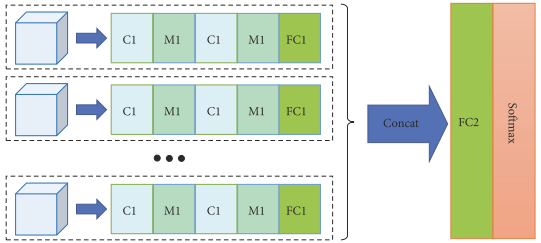
\includegraphics[width=0.7\linewidth]{../HistologicalGradePrediction/images/Yang2019_Fig2}
	\caption{MCF-3DCNN architecture as detailed by \textbf{©Yang et al. \cite{Yang2019}}}
	\label{fig:Yang2019_Figure2_MCF-3DCNN}
\end{figure}


When using a pre-trained architecture, the input size is often dictated
by the native architecture (224x224x3 for example for the ResNet
architecture \cite{Peng2020,WANG2019}), and
the different studies need to resample their inputs to fulfill those
requirements, which can sometimes affect the performances of the
network, whereas custom architectures allow a usage of custom sizes 
\cite{Liang2018,Yasaka2018,Yasaka2018a}. However, 
the size of the lesions or other extracted \ac{roi} is often different 
from one patient to the other, therefore, this problem is still open.\\
One way to render the deep networks robust to those changes is through
multiscale training. Yasaka et al. for example trained the network
with patches cropped at different resolutions from the initial lesion
\ac{roi} after application of standard geometrical transformations
such as rotation or shift \cite{Yasaka2018}. The same
process of extracting different patches from an initial \ac{roi} is performed
by two other studies, where the goal is also to balance the different
classes \cite{Yasaka2018a,Peng2020}.\\
The networks are then usually trained in a cross validation fashion \cite{Yamada2019,Yasaka2018,Yasaka2018a,WANG2019}, or validated on external datasets \cite{Peng2020} to be less affected by the effect of randomness, and to
be less prone to overfitting.

\subsubsection{Performances}\label{performances}

Regarding their performances on their testing sets, the different
studies concluded first that fine tuning allows an improvement in the
accuracy of the \ac{dlr} network, when compared to training from
scratch (e.g. Wang et al. reported an improvement from 83.7 to 91.2\%
regarding the FLL type classification accuracy of their model when using a
pre-trained network) \cite{Wang2018,Yamada2019}. Several studies also demonstrated that multiphase images
increase the performances or the \ac{dlr} networks, when compared to
single phase input only \cite{Yasaka2018}. Instead of
training the \ac{dlr} networks only with images, it is possible to
combine them with clinical data which can be difficult to collect, and
challenging to integrate in a deep architecture, but are proven to
improve the accuracy of the networks in some cases \cite{WANG2019}.\\
Reported results showed moderate to good accuracy for the wanted tasks.
For example, the reported mean accuracy is above 0.90 for the studies
targeting a classification between Focal Nodular Hyperplasias, Cysts,
HCC and Hemangioma (0.91 in both \cite{Liang2018,Wang2018}), and it slightly drops to 0.84 when more complex categories
are integrated (iCC, combined HCC and difference between HCC and early
HCCs) \cite{Yasaka2018a}. Another study performed the
classification between HCCs and non HCCs, by additionally incorporating
the differentiation stages for the HCC group, but still had comparable
performances than experienced radiologists in the diagnostic
performances \cite{Yamada2019}.\\
The study targeting the estimation of the fibrosis stage reported
results less accurate than those obtained using elastography data
(MRE: \emph{Magnetic resonance elastography} or TE: \emph{Transient
elastography}), but they were the first to perform this analysis on CT
images, and their results could be improved with the inclusion of
volumetric information, and other sources of data \cite{Yasaka2018a}.
The only study targeting the prediction of the histological grade using MR images as input was able to correctly classify the \ac{hcc}s into the 3 differentiation groups with a mean accuracy of \textbf{74\%}.\\
Their study however suffers from a lot of limitations such as the
reduced size of the cohort, the imbalanced data and the fact that the
analysis was only performed in a manually drawn \ac{voi} \cite{Yang2019}.\\

Finally, the studies predicting a response to a treatment reported a
high accuracy with an AUC of 0.82 when predicting the recurrence after
TACE \cite{WANG2019}, and accuracy above 0.83 in the two
external validation sets when estimating the response of TACE in HCC
\cite{Peng2020}.\\
Those results still can be improved, especially by increasing the size
of the cohort, or by replacing the manual placement of the bounding
boxes with an automatic segmentation method in order to reduce the
dependency to single or multiple experts \cite{Yasaka2018a,Peng2020}.

As a conclusion, the different reviewed studies tend to agree on the
fact that a multiphase analysis is necessary to precisely describe and
encode the pathological features of the disease. For the rest of the
pipeline, no real consensus exists but several strategies are
implemented especially to compensate for the small size of the
databases. Worth also noting that the reviewed studies correspond to the
first \ac{dlr} liver-related applications, therefore, they tend to tackle the
less complex problems such as the \ac{fll}s classification. We believe that currently, when only a small amount of data is available, and when the differentiation can be performed using simple criteria, then an HCR-based pipeline will be superior to a DLR one. With future
improvements regarding \ac{dl} applied to the medical imaging field, and with more publicly available data, the next \ac{dlr} liver-related studies will be ready to tackle more complex challenges.\\
In our research work, we conducted a study aiming for the histological grade prediction, 
consequently, we designed a pipeline following the aforementioned conclusions. 
The key element in our work was an automatic cascaded liver and tumor segmentation performed on registered multiphase CT images. It is worth noting that we are the first to perform prediction of the histological grade from multiphase CT images using a fully automatic pipeline. 
